\documentclass[cs4size,a4paper,10pt]{ctexart}   

\linespread{1.5}
\usepackage{geometry}%用于设置上下左右页边距
	\geometry{left=2.5cm,right=2.5cm,top=3.2cm,bottom=2.7cm}
\usepackage{xeCJK,amsmath,paralist,enumerate,booktabs,multirow,graphicx,subfig,setspace,listings,lastpage,hyperref}
\usepackage{amsthm, amssymb, bm, color, framed, graphicx, hyperref, mathrsfs}
\usepackage{mathrsfs}  
	\setlength{\parindent}{2em}
	\lstset{language=Matlab}%
\usepackage{fancyhdr}
\usepackage{graphicx}
\usepackage{subfloat}
\usepackage{listings}
\usepackage{xcolor}
\usepackage{float}
\usepackage{paralist}
\usepackage{setspace}
\usepackage{titlesec}
\usepackage{enumitem}
\usepackage{hyperref}
\usepackage{multirow}
\usepackage{threeparttable}
\usepackage{autobreak}
\usepackage{multicol}
\usepackage{subfig}


\hypersetup{
	colorlinks=true,
	linkcolor=black,
	urlcolor=black
}

\setenumerate{partopsep=0pt,topsep=0pt}
\setitemize{itemsep=0pt,partopsep=0pt,topsep=0pt}

\titlespacing*{\section}{0pt}{3pt}{3pt}
\titlespacing*{\subsection}{0pt}{2pt}{2pt}
\titlespacing*{\subsubsection}{0pt}{1pt}{1pt}
\titlespacing*{\paragraph}{0pt}{0pt}{0pt}

\ctexset{secnumdepth=4,tocdepth=4}
\setlength{\parindent}{0pt}
\setstretch{1.2}


\setCJKmainfont[BoldFont={FZHei-B01},ItalicFont={FZKai-Z03}]{FZShuSong-Z01} 
\setCJKsansfont[BoldFont={FZHei-B01}]{FZKai-Z03} 
\setCJKmonofont[BoldFont={FZHei-B01}]{FZFangSong-Z02}
\setCJKfamilyfont{zhsong}{FZShuSong-Z01} 
\setCJKfamilyfont{zhhei}{FZHei-B01} 
\setCJKfamilyfont{zhkai}[BoldFont={FZHei-B01}]{FZKai-Z03} 
\setCJKfamilyfont{zhfs}[BoldFont={FZHei-B01}]{FZFangSong-Z02} 
\renewcommand*{\songti}{\CJKfamily{zhsong}} 
\renewcommand*{\heiti}{\CJKfamily{zhhei}} 
\renewcommand*{\kaishu}{\CJKfamily{zhkai}} 
\renewcommand*{\fangsong}{\CJKfamily{zhfs}}


\definecolor{mKeyword}{RGB}{0,0,255}          % bule
\definecolor{mString}{RGB}{160,32,240}        % purple
\definecolor{mComment}{RGB}{34,139,34}        % green
\definecolor{mNumber}{RGB}{128,128,128} 

\lstdefinestyle {njulisting} {
	basewidth = 0.5 em,
	lineskip = 3 pt,
	basicstyle = \small\ttfamily,
	% keywordstyle = \bfseries,
	commentstyle = \itshape\color{gray}, 
	basicstyle=\small\ttfamily,
	keywordstyle={\color{mKeyword}},     % sets color for keywords
	stringstyle={\color{mString}},       % sets color for strings
	commentstyle={\color{mComment}},     % sets color for comments
	numberstyle=\tiny\color{mNumber},
	numbers = left,
	captionpos = t,
	breaklines = true,
	xleftmargin = 2 em,
	xrightmargin = 2 em,
	frame=tlrb,
	tabsize=4
}

\lstset{
style = njulisting, % 调用上述样式 
flexiblecolumns % 允许调整字符宽度
}


%================= 基本格式预置 ===========================
\usepackage{fancyhdr}
\pagestyle{fancy}
\lhead{\textsc{Automated Testing}}
\rhead{自动化测试期末复习}
\cfoot{\thepage}
\renewcommand{\headrulewidth}{0.4pt}
\renewcommand{\theenumi}{(\arabic{enumi})}
\CTEXsetup[format={\bfseries\zihao{-3}}]{section}
\CTEXsetup[format={\bfseries\zihao{4}}]{subsection}
\CTEXsetup[format={\bfseries\zihao{-4}}]{subsubsection}


\renewcommand{\contentsname}{目录}  
\begin{document}

	\begin{center}
		{\huge\textbf{自动化测试期末复习}}
	\end{center}
	%---------目录---------% 
	\pagenumbering{Roman}
	\tableofcontents
	\clearpage

 	%---------正文---------% 
	\pagenumbering{arabic}
	\setcounter{page}{1}
	\setlength{\parskip}{0.65em}
	
	\section{源码测试}

\subsection{随机测试}
\begin{figure}[H]
    \vspace{-0.5em}
	\centering
	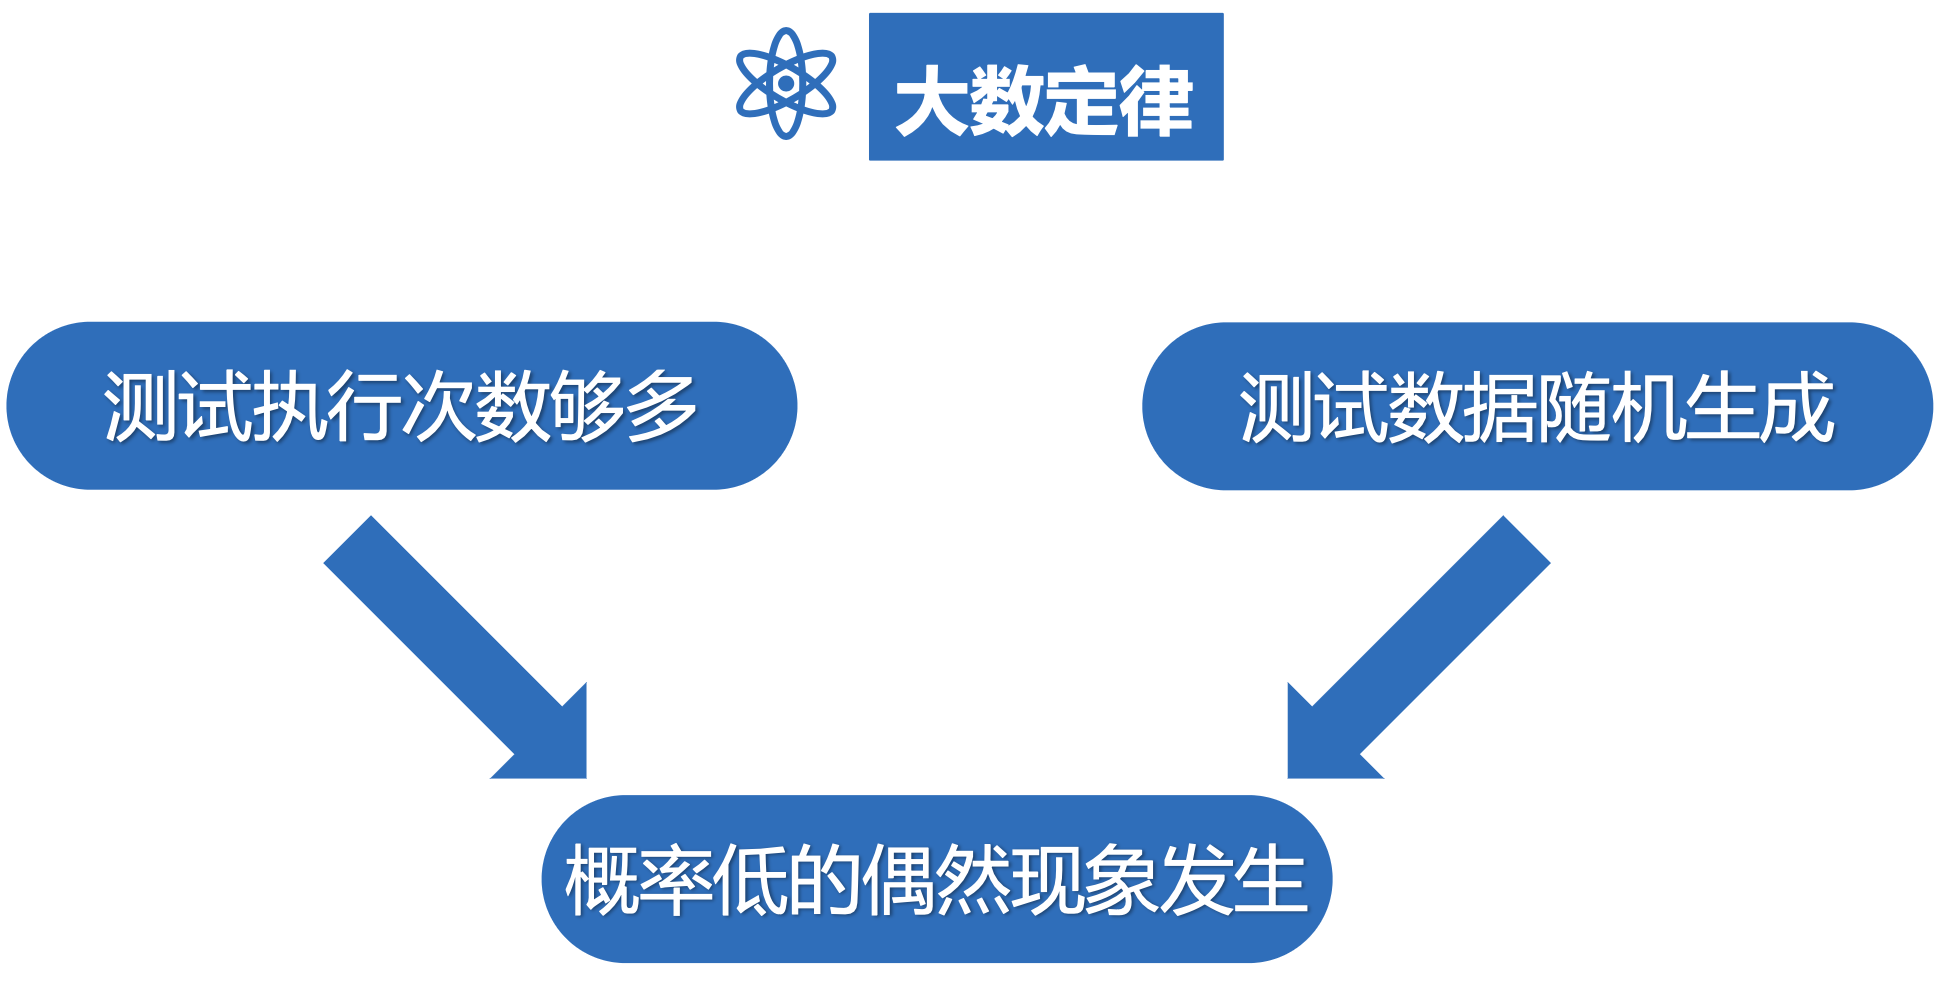
\includegraphics[width=0.5\textwidth]{images/随机测试.png}
    \vspace{-1em}
\end{figure}

\subsection{变异测试}
变异测试旨在找出有效的测试用例,发现程序中真正的错误。
\begin{figure}[H]
    \vspace{-0.5em}
	\centering
	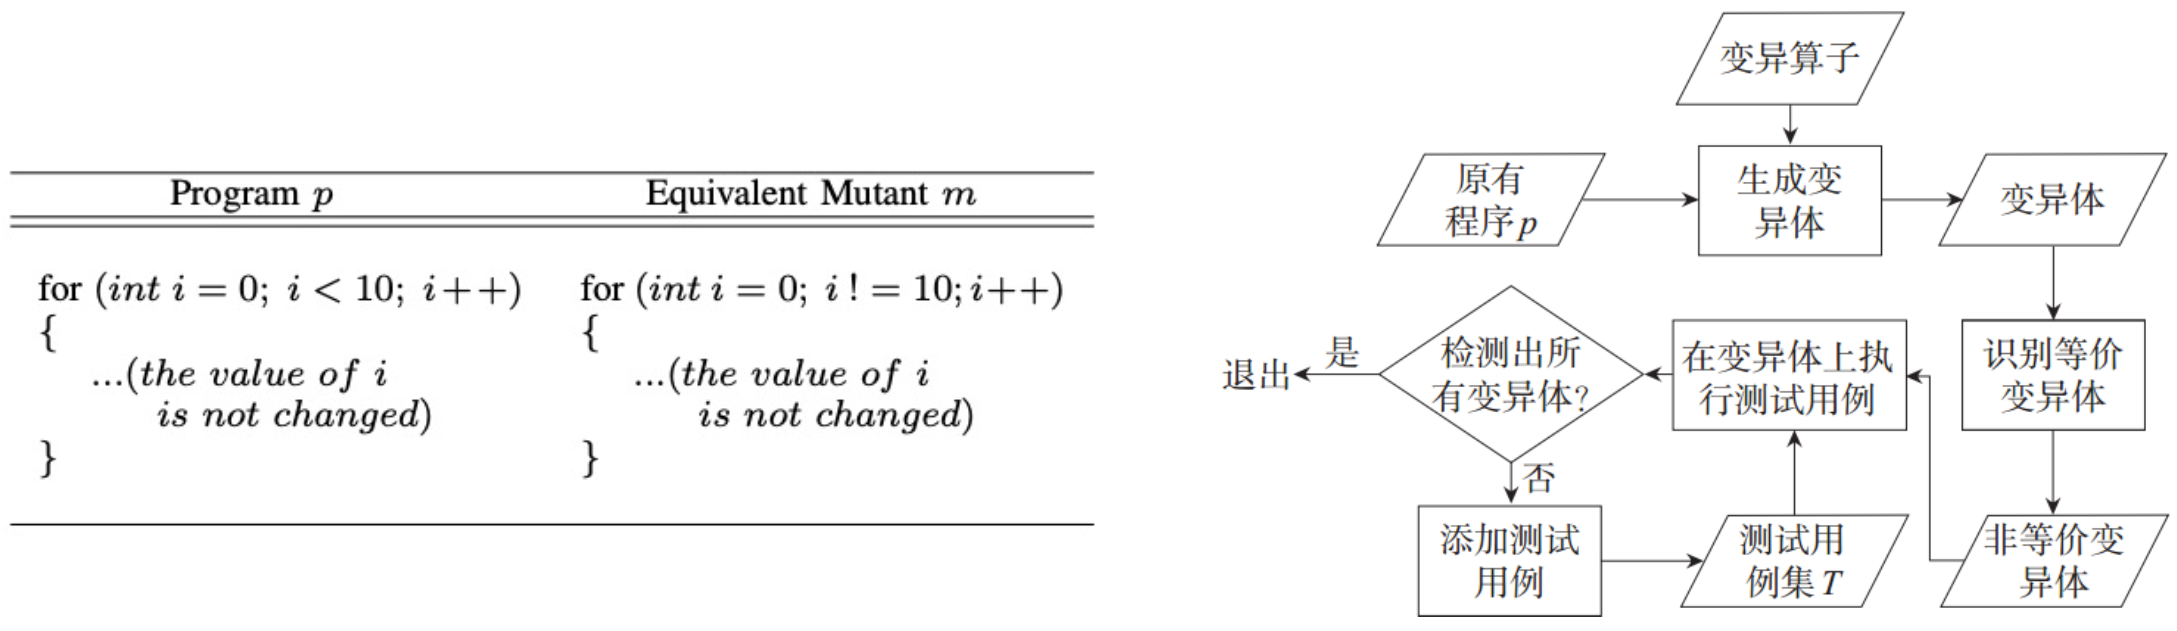
\includegraphics[width=0.95\textwidth]{images/变异测试.png}
    \vspace{-1em}
\end{figure}

\subsection{差分测试}
基本思想:通过将同一测试用例运行到一系列相似功能的应用中观察执行差异来检测bug。
\begin{figure}[H]
    \vspace{-0.5em}
	\centering
	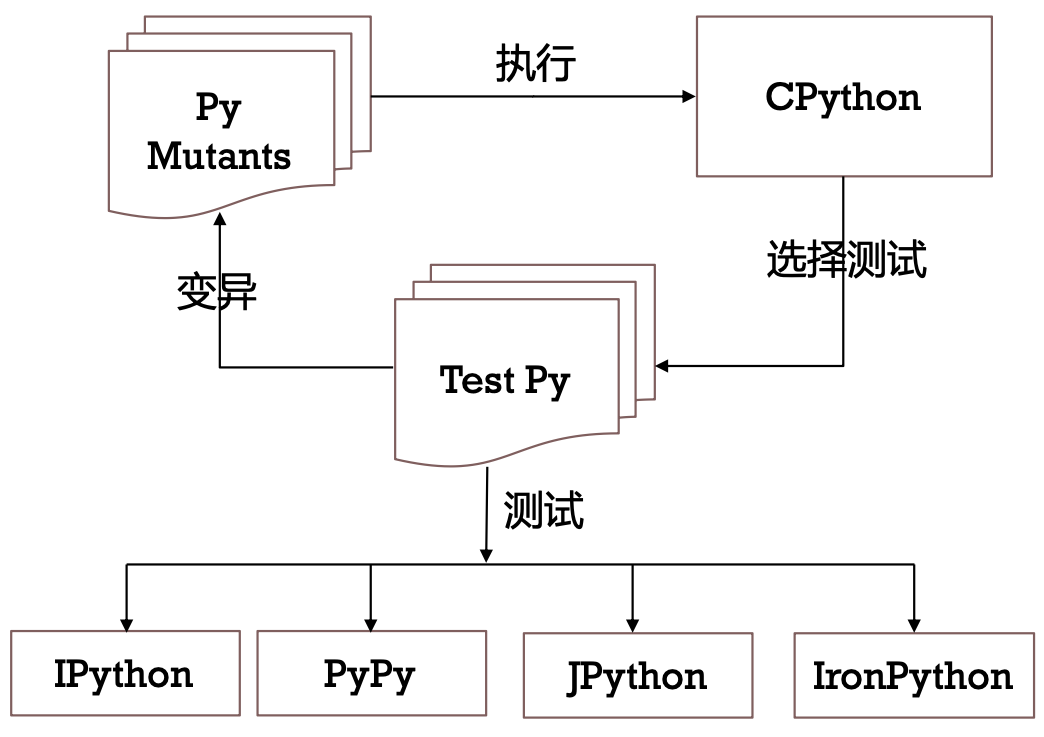
\includegraphics[width=0.4\textwidth]{images/差分测试.png}
    \vspace{-1em}
\end{figure}

\subsection{蜕变测试}
蜕变关系(Metamorphic Relation, MR)是指多次执行目标程序时,输入与输出之间期望遵循的关系。
\begin{figure}[H]
    \vspace{-0.5em}
	\centering
	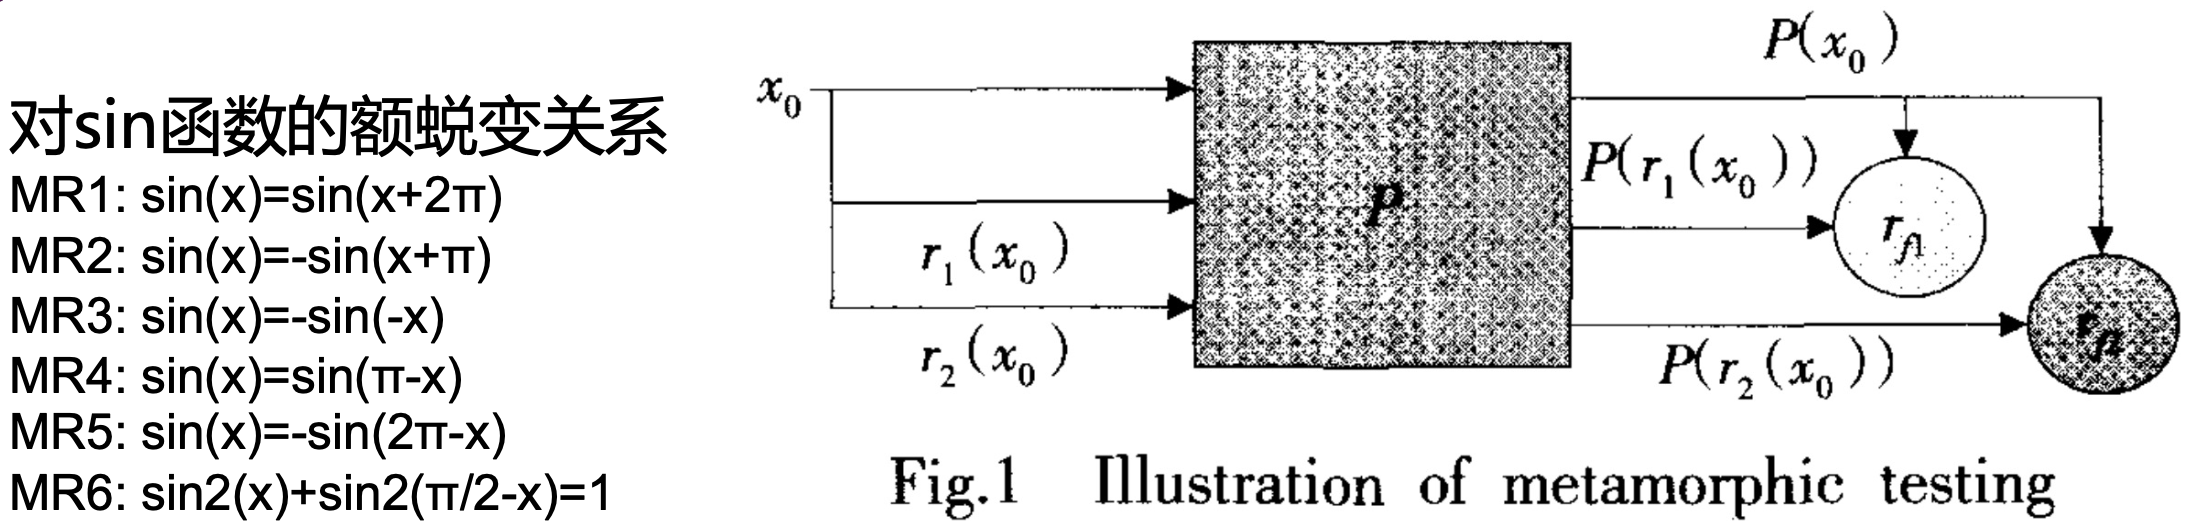
\includegraphics[width=0.75\textwidth]{images/蜕变测试.png}
    \vspace{-1em}
\end{figure}

\subsection{测试用例优先级(TCP)}

测试用例优先级的定义:通过设定特定优先级准则(执行时间,代码覆盖等),对测试用例进行优先级排序以优化其执行次序,旨在最大化优先级目标,例如最大化测试用例集的早期缺陷检测速率。

优先级策略:
\begin{itemize}
    \item 基于贪心的TCP策略
    \item 基于相似性的TCP策略
    \item 基于搜索的TCP策略
    \item 基于机器学习的TCP策略
\end{itemize}

\subsubsection{基于贪心的TCP策略}

\begin{itemize}
    \item 全局贪心策略
    \begin{itemize}
        \item 每轮优先挑选覆盖最多代码单元的测试用例
        \item 多个用例相同随机选择
    \end{itemize}
    \item 增量贪心策略
    \begin{itemize}
        \item 每轮优先挑选覆盖最多,且\textbf{未被已选择用例覆盖代码}单元的测试用例
        \item 所有代码单元均已被覆盖则重置优先级排序过程
        \item 多个用例相同随机选择
    \end{itemize}
\end{itemize}

\begin{figure}[H]
    \vspace{-0.5em}
	\centering
	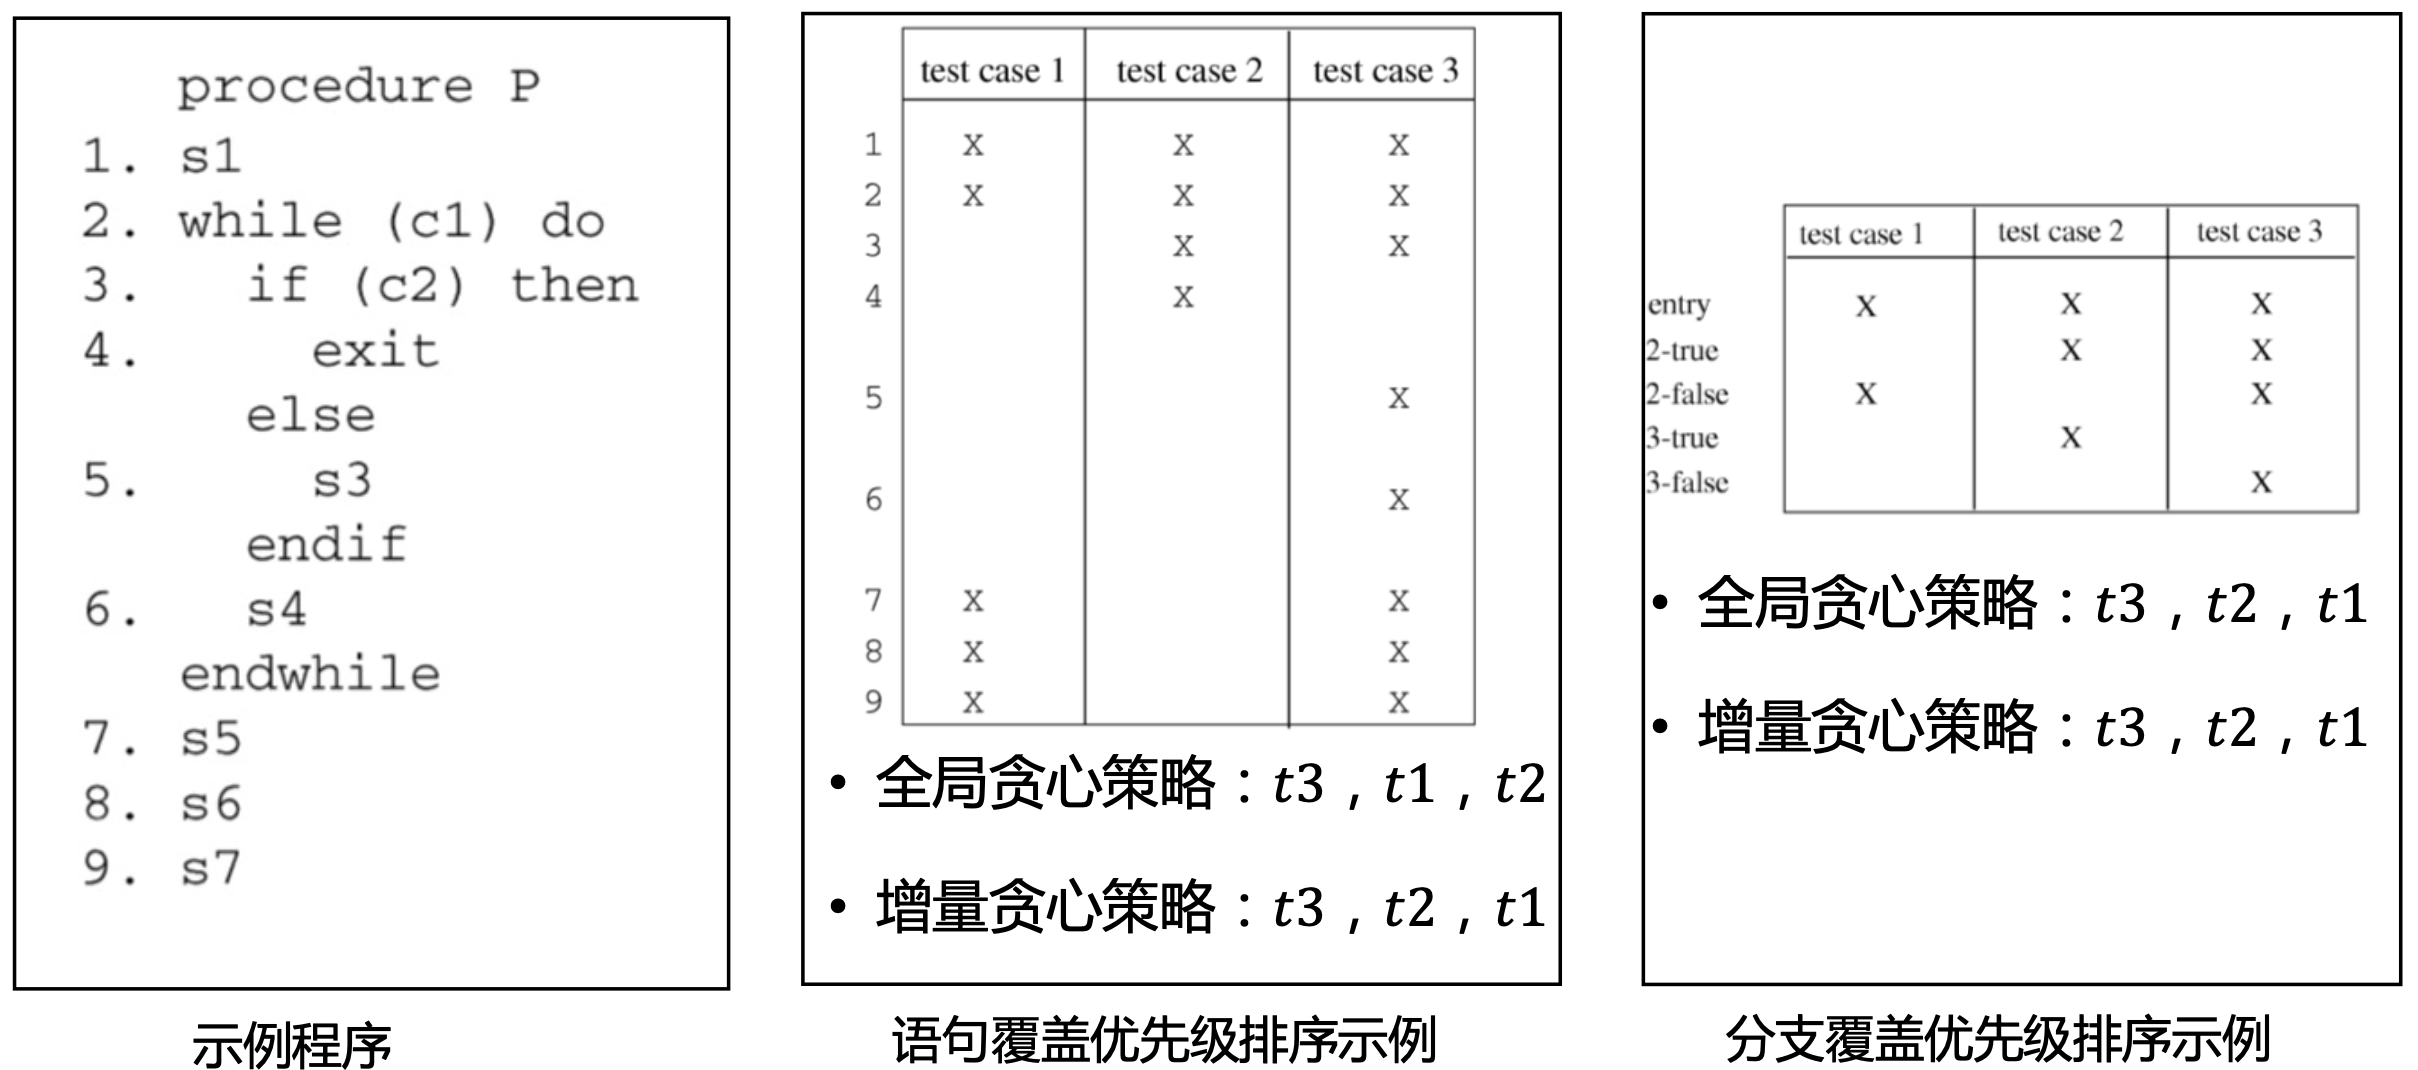
\includegraphics[width=0.8\textwidth]{images/基于贪心的TCP策略.png}
    \vspace{-1em}
\end{figure}

计算过程:
\begin{enumerate}[label=\arabic*.]
    \item 初始化覆盖矩阵和语句覆盖数组,所有代码单元均未被覆盖,$c$为全0数组
    \begin{figure}[H]
        \vspace{-0.5em}
        \centering
        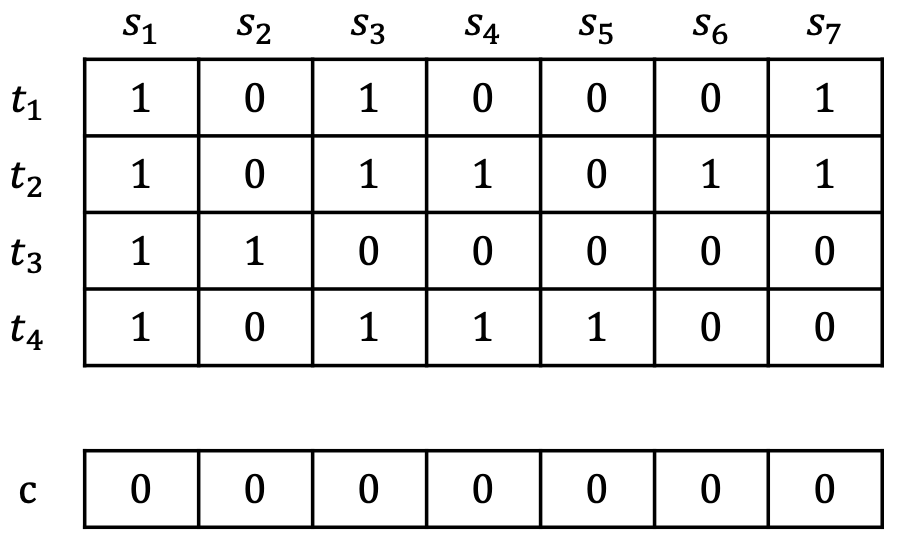
\includegraphics[width=0.3\textwidth]{images/基于贪心的TCP策略计算过程.png}
        \vspace{-1em}
    \end{figure}
    \item 根据覆盖矩阵和单元覆盖数组,计算待排序用例覆盖值,选择测试用例
    \item 选择测试用例,更新语句覆盖数组,以及待排序测试用例覆盖值
    \item 重复上述步骤,当所有语句均被覆盖时,重置语句覆盖数组,计算剩余测试用例覆盖值
\end{enumerate}

假设有$n$个测试用例以及$m$个代码单元,共需排序$n$轮,每轮选择一个测试用例,第$k$轮时,存在$n-k+1$个待排序用例,每个用例需与$m$个代码单元计算情况,那么时间复杂度为$O(n^2m)$。

\subsubsection{基于相似性的TCP策略}
自适应随机策略:每轮优先与已选择测试用例集差异性最大的测试用例。让测试用例均匀地分布在输入域中。

测试用例之间的距离计算:假设$U(t_1)$和$U(t_2)$为测试用例$t_1$和$t_2$所覆盖的代码单元集合,那么这两个用例之问的距离计算如下:
$$Jaccard(t_1, t_2) = 1-\frac{|U(t_1) \cap U(t_2)|}{|U(t_1) \cup U(t_2)|}$$

测试用例与测试用例集之间的距离计算:分别使用最小距离、平均距离和最大距离度量方式计算待选择用例$t_c$与已选择用例集$S$的距离:
$$
D(t_c, S) = \left\{ \begin{array}{c}
    \max\{\min\limits_{0\leq i \leq |S|} \{Jaccard(t_c,t_i)\}\} \\
    \max\{\mathop{\mathrm{avg}}\limits _{0\leq i \leq |S|} \{Jaccard(t_c,t_i)\}\} \\
    \max\{\max\limits_{0\leq i \leq |S|} \{Jaccard(t_c,t_i)\}\} \\
\end{array}\right.
$$

\begin{figure}[H]
    \vspace{-0.5em}
	\centering
	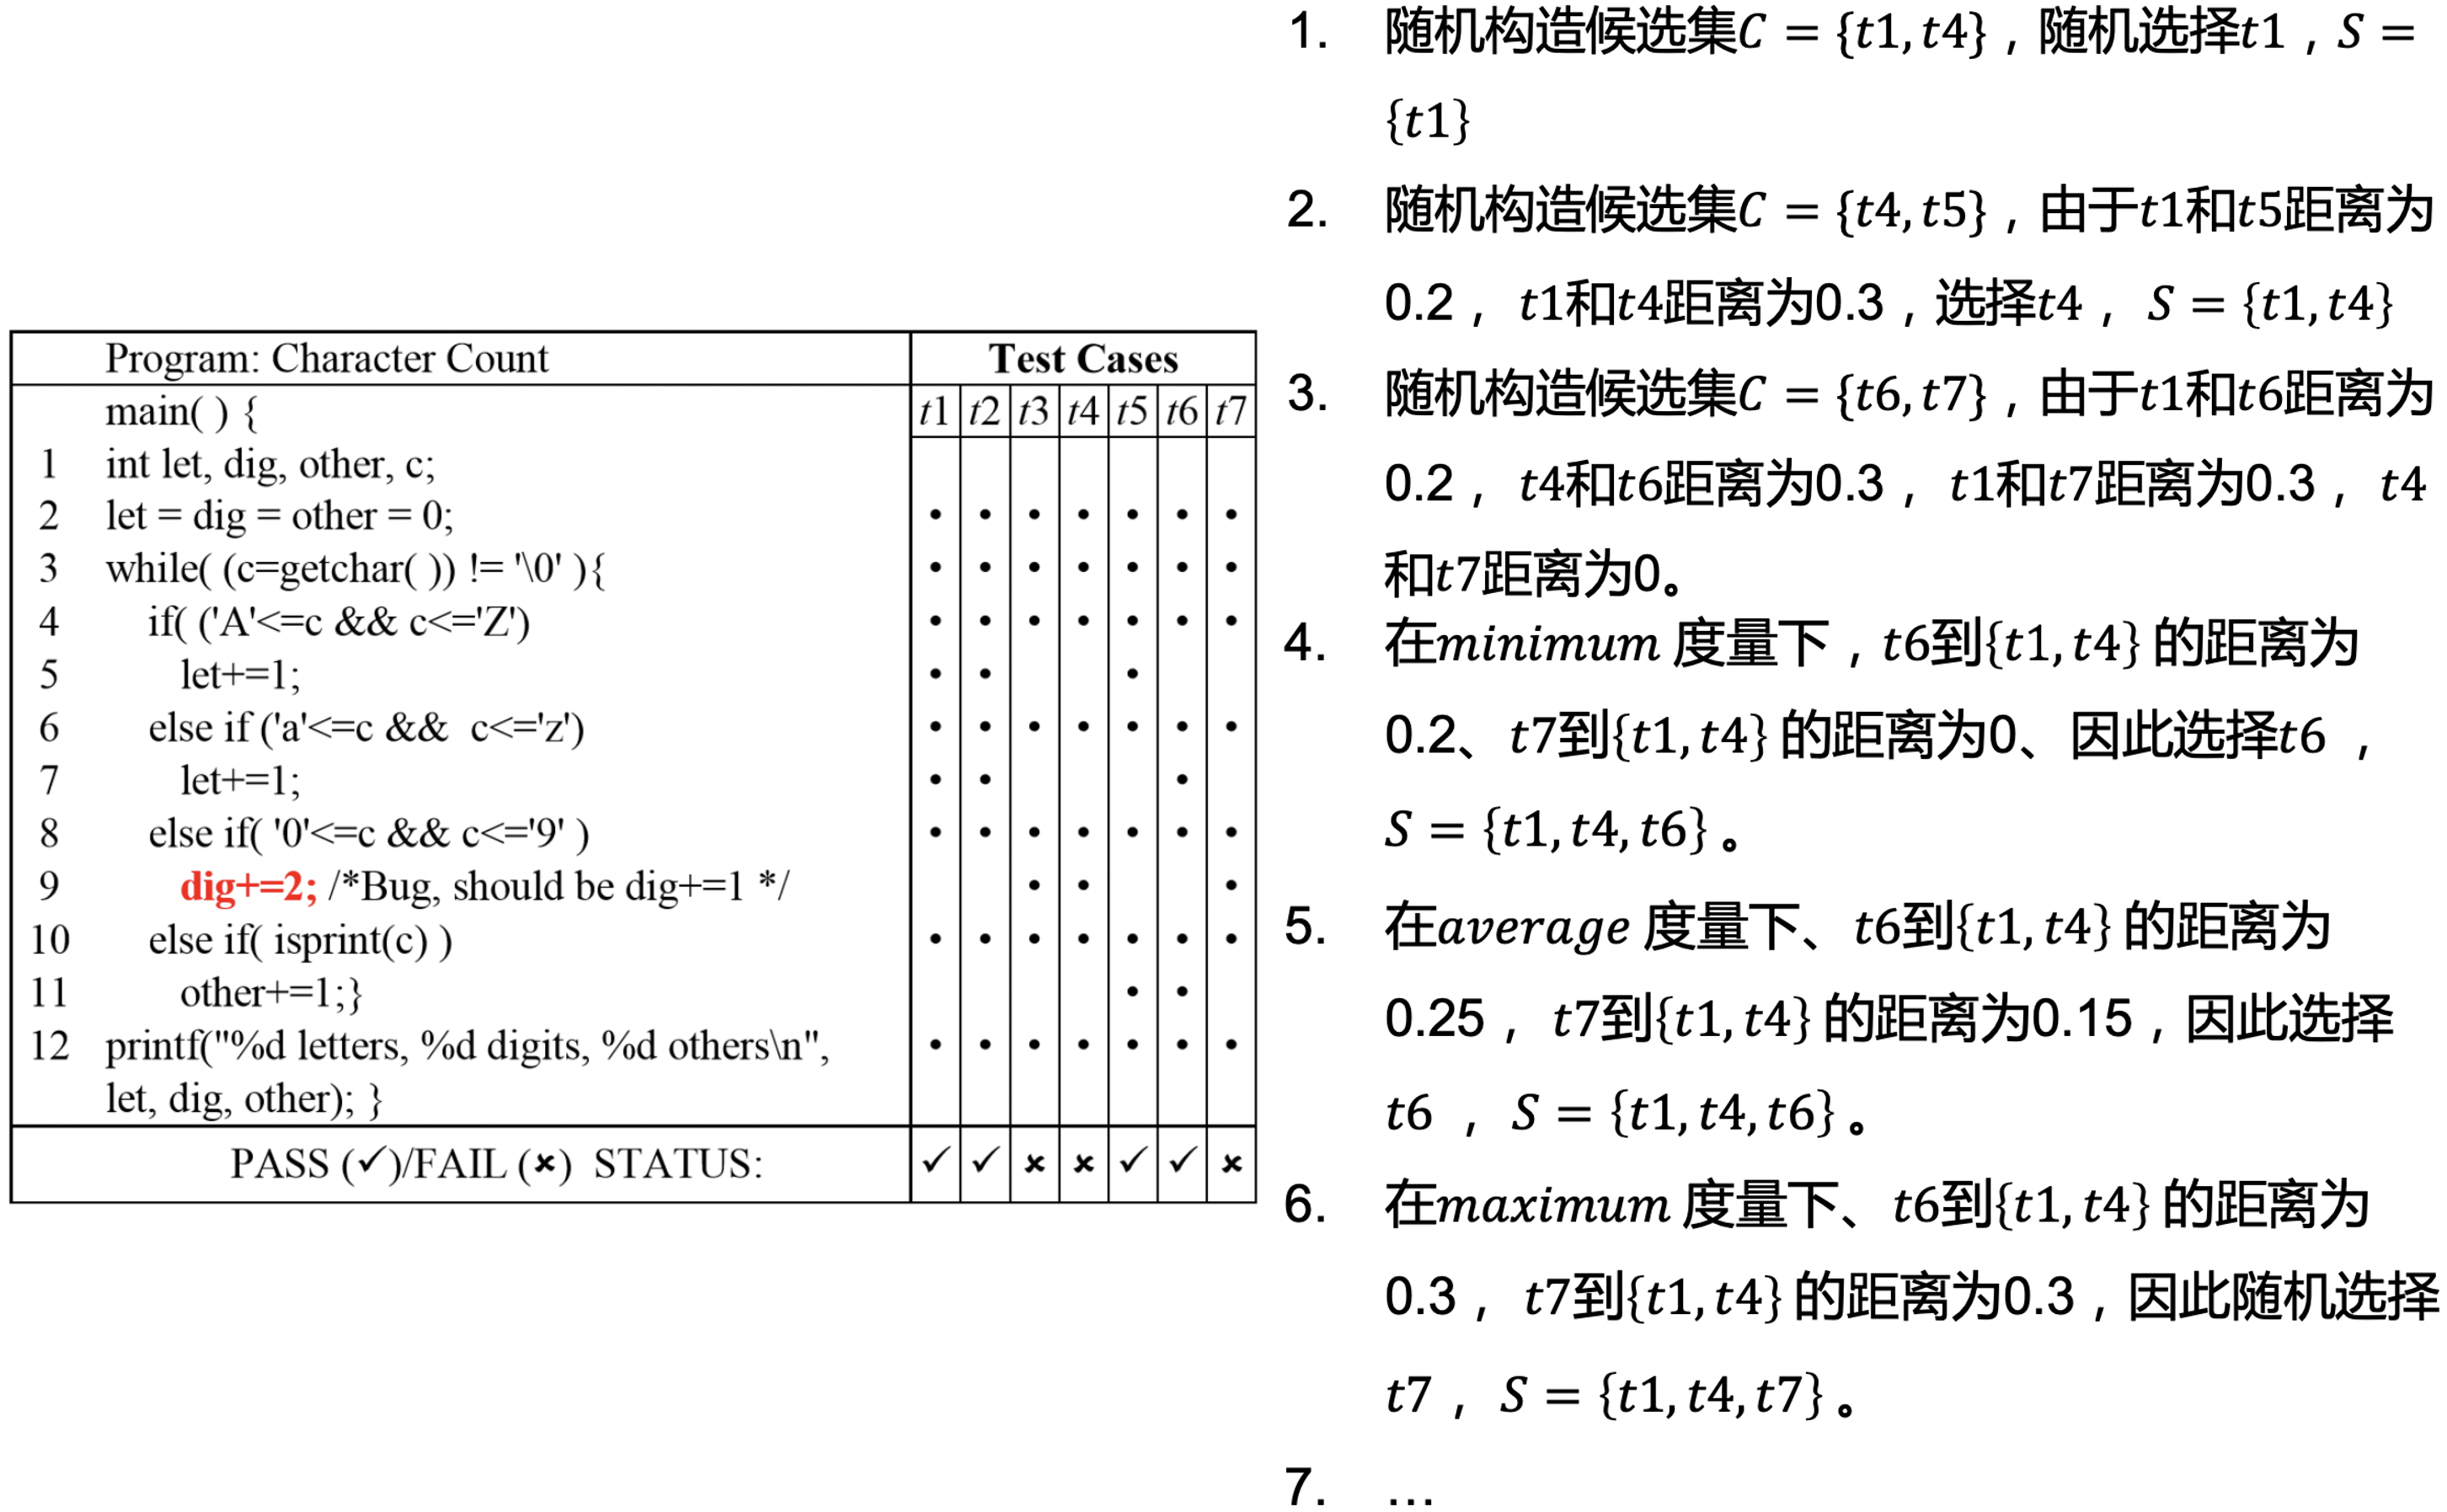
\includegraphics[width=0.75\textwidth]{images/基于相似性的TCP策略.png}
    \vspace{-1em}
\end{figure}

\subsubsection{基于搜索的TCP策略}
探索用例优先级排序组合的状态空间,以此找到检测错误更快的用例序列
\begin{itemize}
    \item 初始种群构造:测试用例位置构成解编码形式。
    \item 交叉操作:使用单点交叉方式,交换两个用例切割点前后部分。
    \item 变异操作:随机选取个体中的两个基因座进行交换。
    \item 适应度评估:使用用例序列的覆盖代码单元速率进行评估
\end{itemize}

\subsubsection{基于机器学习的TCP策略}
对测试用例特征进行学习,根据预测的缺陷检测概率进行优先级排序。
\begin{enumerate}[label=\arabic*.]
    \item 特征提取:设计并提取测试程序中源码特征。
    \item 缺陷模型:建立模型预测测试程序检测缺陷的概率。
    \item 开销模型:建立模型预测测试程序的运行时问。
    \item 测试优先级:基于单位时间内检测缺陷能力进行优先级排序。
\end{enumerate}

\subsubsection{APFD计算}
APFD的一般性描述:给定程序包含$m$个故障$F=\{f_1,f_2,\cdots, f_m\}$和$n$个测试用例$T=\{t_1,t_2,\cdots, t_n\}$,$T^ \prime$为$T$的一个优先级序列,$TF_i$为该测试用例序列$T^ \prime$中第一个检测到故障$f_i$的测试用例下标,则该优先级序列$T^ \prime$的APFD值计算公式为
$$APFD=1- \frac{TF_1 + TF_2 +\cdots + TF_m}{n\times m} + \frac{1}{2n}$$

\begin{figure}[H]
    \vspace{-0.5em}
	\centering
	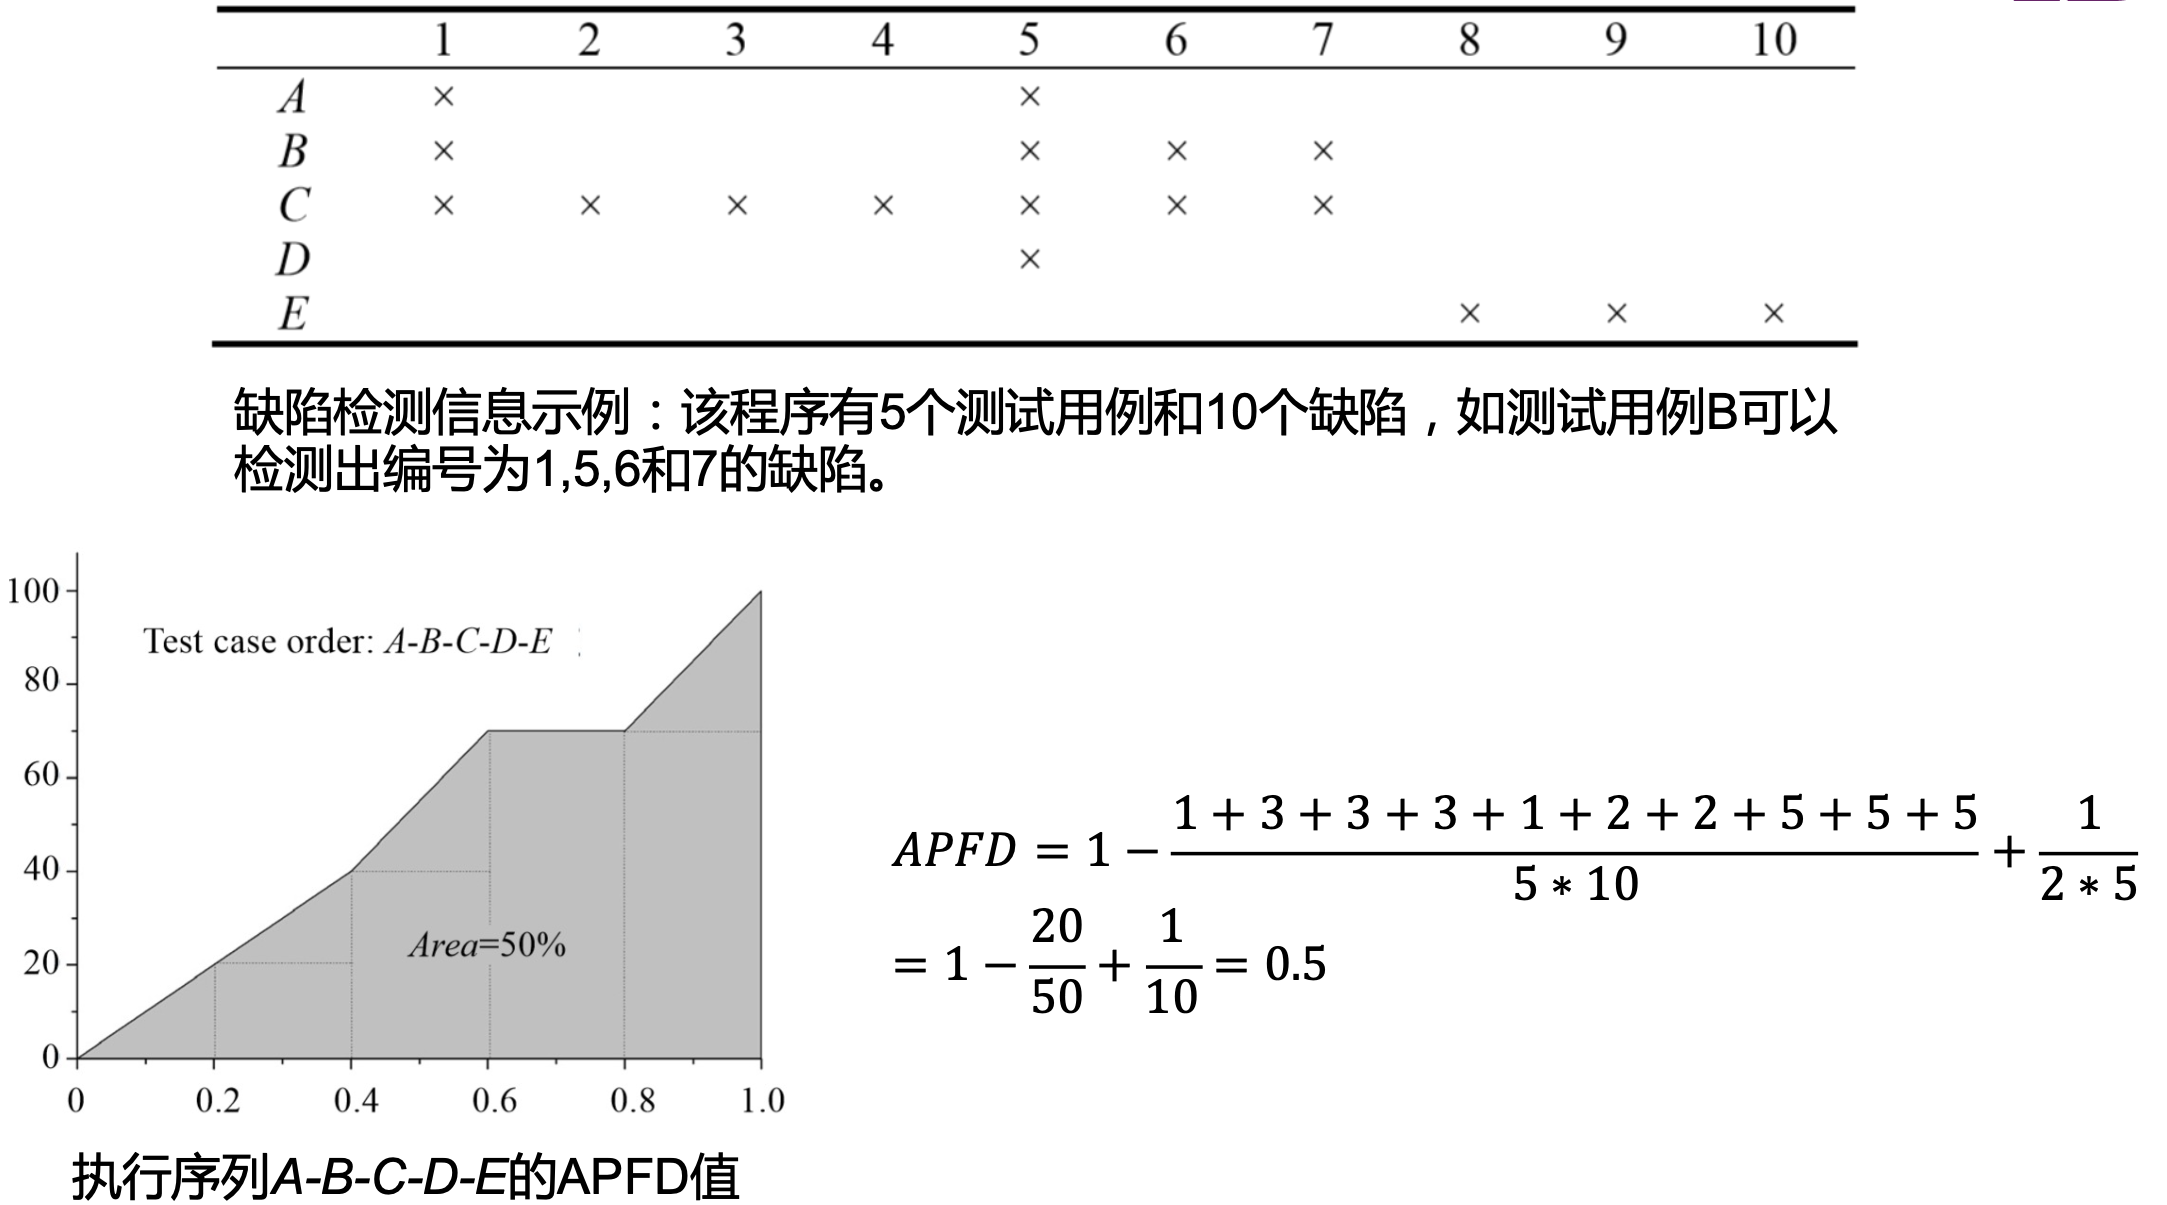
\includegraphics[width=0.8\textwidth]{images/APFD.png}
    \vspace{-1em}
\end{figure}

\subsection{测试用例选择(TCS)}
TCS定义:旨在从已有测试用例集中选择出所有可检测代码修改的测试用例。

适用场景:适用于因测试预算不足以致不能执行完所有测试用例的测试场景。

测试选择是回归测试选择的核心环节
\begin{itemize}
    \item 测试选择可以依照某种策略,从测试全集中筛选出一个子集。通过重新运行这个一个子集,验证版本迭代是否对软件既有的某些功能造成了影响。
    \item 给定修改前的生产代码$P$、修改后的生产代码$P^\prime$以及测试全集$T$,测试选择就是根据某种选择策略$S$,从$T$中筛选出测试子集$T^\prime$,使$T^\prime$能够评估代码变更是否影响了程序的既有功能。
\end{itemize}

根据不同的选取策略,测试用例选择可大致分为以下四类
\begin{itemize}
    \item 最小化测试用例选择技术
    \begin{itemize}
        \item 目标:从原测试套件$T$中选出最少的测试用例组成最小最小测试集$T_{min}$ ,使得产生的$T_{min}$能多覆盖被测程序$P$中所有本次修改的、或者受本次修改影响的部分。
        \item 要求:一个最小化测试用例选择技术要求修改后的被测试程序$P$中,每一条新增的或者被修改的语句都能够被至少一个来自原测试套件$T$的测试用例执行。
    \end{itemize}
    \item 安全测试用例选择技术
    \begin{itemize}
        \item 目标:针对某种特定的测试需求,选取出源测试套件$T$中所有能够暴露修改后被测程序$P^\prime$中的一个或多个缺陷的所有测试用例,构成安全回归测试集$T_S$。
        \item 一个安全测试用例选择技术要求在目标程序$P$运行回归测试时,$T_S$中的每个测试都能够满足以下条件之一:
        \begin{itemize}
            \item 执行至少一条在$P^\prime$中被删除的语句
            \item 执行至少一条在$P^\prime$中新增的语句
        \end{itemize}
    \end{itemize}
    \item 基于数据流和覆盖的测试用例选择技术
    \begin{itemize}
        \item 目标:当代码变更发生后,原待测程序$P$更新为$P^\prime$。相比于$P$,$P^\prime$中部分语句的数据交互发生了变化。这些发生变化的语句构成了语句集合$S_I$。基于数据流和覆盖的测试用例选择技术的目标是选取出所有能够执行到$S_I$中某条语句的测试用例,组成测试集$T_D$。
        \item 要求:一个安全测试用例选择技术要求在目标程序$P$运行回归测试时,$T_D$中的每个测试都能够满足以下条件之一:
        \begin{itemize}
            \item 执行至少一个在$P^\prime$中被删除的Define-Use对
            \item 执行至少一个在$P^\prime$中新增的Define-Use对
        \end{itemize}
    \end{itemize}
    \item 特制/随机测试用例选择技术
    \begin{itemize}
        \item 定义:当时间不允许使用ReTestAl策略进行回归测试、且没有任何可用的测试用例选择工具时,开发人员通常会依赖“直觉"或者测试与生产代码功能之间的弱关联进行测试用例选择。
        \item 举例:
        \begin{itemize}
            \item 随机测试用例选择:规定测试用例的选取数量为$m$ ,测试人员随机地从原始测试套件$T$选出$m$个测试用例,组成随机回归测试集$T_R$
            \item 面向剖面测试用例选择:与面向剖面程序编程有关,从原始测试套件$T$中选出与某个剖面$a$有关的化测试用例,组成回归测试集$T_a$
        \end{itemize}
    \end{itemize}
\end{itemize}

\subsection{基于程序分析的测试选择}
一种依赖程序分析的测试选择技术。该技术一般通过程序分析技术计算测试代码(方法、用例或套件)与生产代码之间存在的依赖关系,井在代码发生变更时,利用这些依赖关系将所有受到变更影响的测试代码自动选取出来,组成测试子集。

\begin{itemize}
    \item 静态测试选择:以静态程序分析为基础实现的测试选择技术。静态(程序)分析是指在没有实际执行程序的情况下对计算机软件程序进行自动化分析的技术。
    \item 动态测试选择:以动态程序分析为基础实现的测试选择技术。动态(程序)分析通过在真实或虚拟处理器上执行程序来完成对程序行为的分析。为了使动态程序分析有效,此须使用足够的测试输人来执行目标程序,以尽可能覆盖程序所有的输出。
\end{itemize}

对比动态测试用例选择和静态测试用例选择
\begin{itemize}
    \item 总体:动态测试用例选择>静态测试用例选择。
    \item 以面向Java语言的测试用例选择技术为例,动态测试用例选择技术一般要优于静态测试用例选择技术,原因在于:动态分析能够更容易地获得更加丰富的(运行时信息)程序依赖信息,测试用例选择更加精准、安全;而相比之下静态分析的开销更大,同时存在过拟合现象。
    \item 静态测试用例选择技术在运行测试阶段的表现一般要优于动态测试用例选择技术,其原因在于静态分析不需要对代码进行插桩 ,在执行代码前就能够获得测试用例选择所需的测试依赖。
\end{itemize}

类防火墙算法:所有能够通过继承边或使用边直接或间接到达某些发生变更类型的类型的集合
\begin{itemize}
    \item 给定一组变更的类,类防火墙将利用类之间的关系计算其他可能受变更影响的一组类,即围绕变更的类构建“防火墙”
\end{itemize}
\begin{figure}[H]
    \vspace{-0.5em}
	\centering
	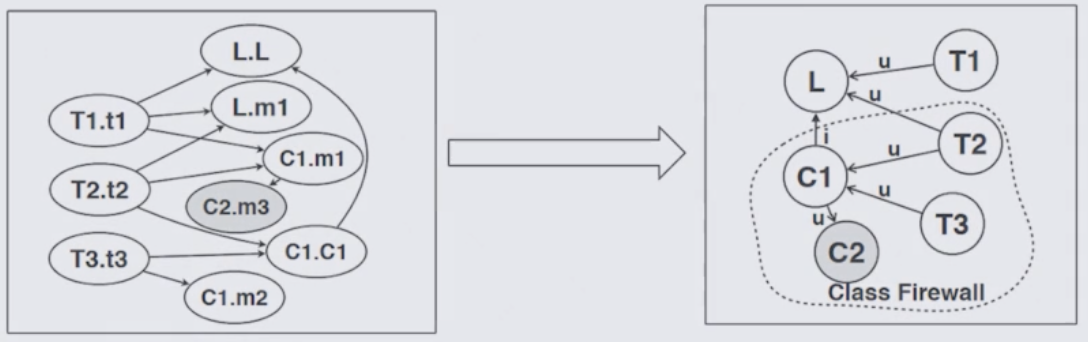
\includegraphics[width=0.6\textwidth]{images/类防火墙.png}
    \vspace{-1em}
\end{figure}

回归测试优先选择:
\begin{enumerate}[label=\arabic*.]
    \item 新修改的功能,这个显然是重点;
    \item 新修改的功能的关联功能,就是有耦合的部分,这个一般最好咨询一下开发人员;
    \item 程序最有卖点或者说亮点的部分,这个地方一旦有问题,会使程序质量大打折扣;
    \item 程序中最致命的部分,譬如说安全隐患,数据泄露,加密注册;
    \item 程序中比较脆弱的部分,这个要咨询开发人员,一般就是他们心中最没底的地方;
    \item 程序的主干功能;
    \item 如果以上做完,还有时间的话,最好把用例中级别比较高的用例再执行一遍。
\end{enumerate}

\subsection{TCP和TCS的对比}
测试用例选择:通过分析代码修改,从已有测试用例中选择出所有可检测代码修改的测试用例,并确保未被选择的测试用例在修改前后程序上的执行行为保持一致。

测试用例优先级:当测试预算不足以执行完所有测试用例时,基于特定的优先级准则,对测试用例进行优先级排序,以优化其执行次序,旨在最大化优先级目标。


	\section{基于图像理解的移动应用自动化测试}

移动应用自动化测试的难点:移动应用碎片化
\begin{itemize}
    \item 不同的操作系统,不同的打开方式都会让页面呈现不同的效果,这使得测试脚本不能简单地复制粘贴使用。
\end{itemize}

录制回放的可能性:尽管在某些具体推荐内容、地址栏等地方不一致,但整体布局和功能上是相似的。

\begin{itemize}
    \item GUI测试脚本录制:
    \begin{itemize}
        \item 基于坐标:录制内容为用户的动作和相应的点击坐标
        \item 基于控件树:主流方法,对UI控件树进行解析,以控件的唯一标识(如xpath)对控件进行定位
        \item 基于图像:对比控件截图与屏幕截图从当前UI中定位控件
    \end{itemize}
    \item GUI测试脚本录制与回放:
    \begin{itemize}
        \item 大多数移动应用在不同平台上设计的UI布局结构极为相似,因此可以利用这种相似性进行移动应用的GUI测试脚本录制与回放
    \end{itemize}
\end{itemize}

\subsection{脚本录制与回放的基本框架}
\begin{figure}[H]
    \vspace{-0.5em}
	\centering
	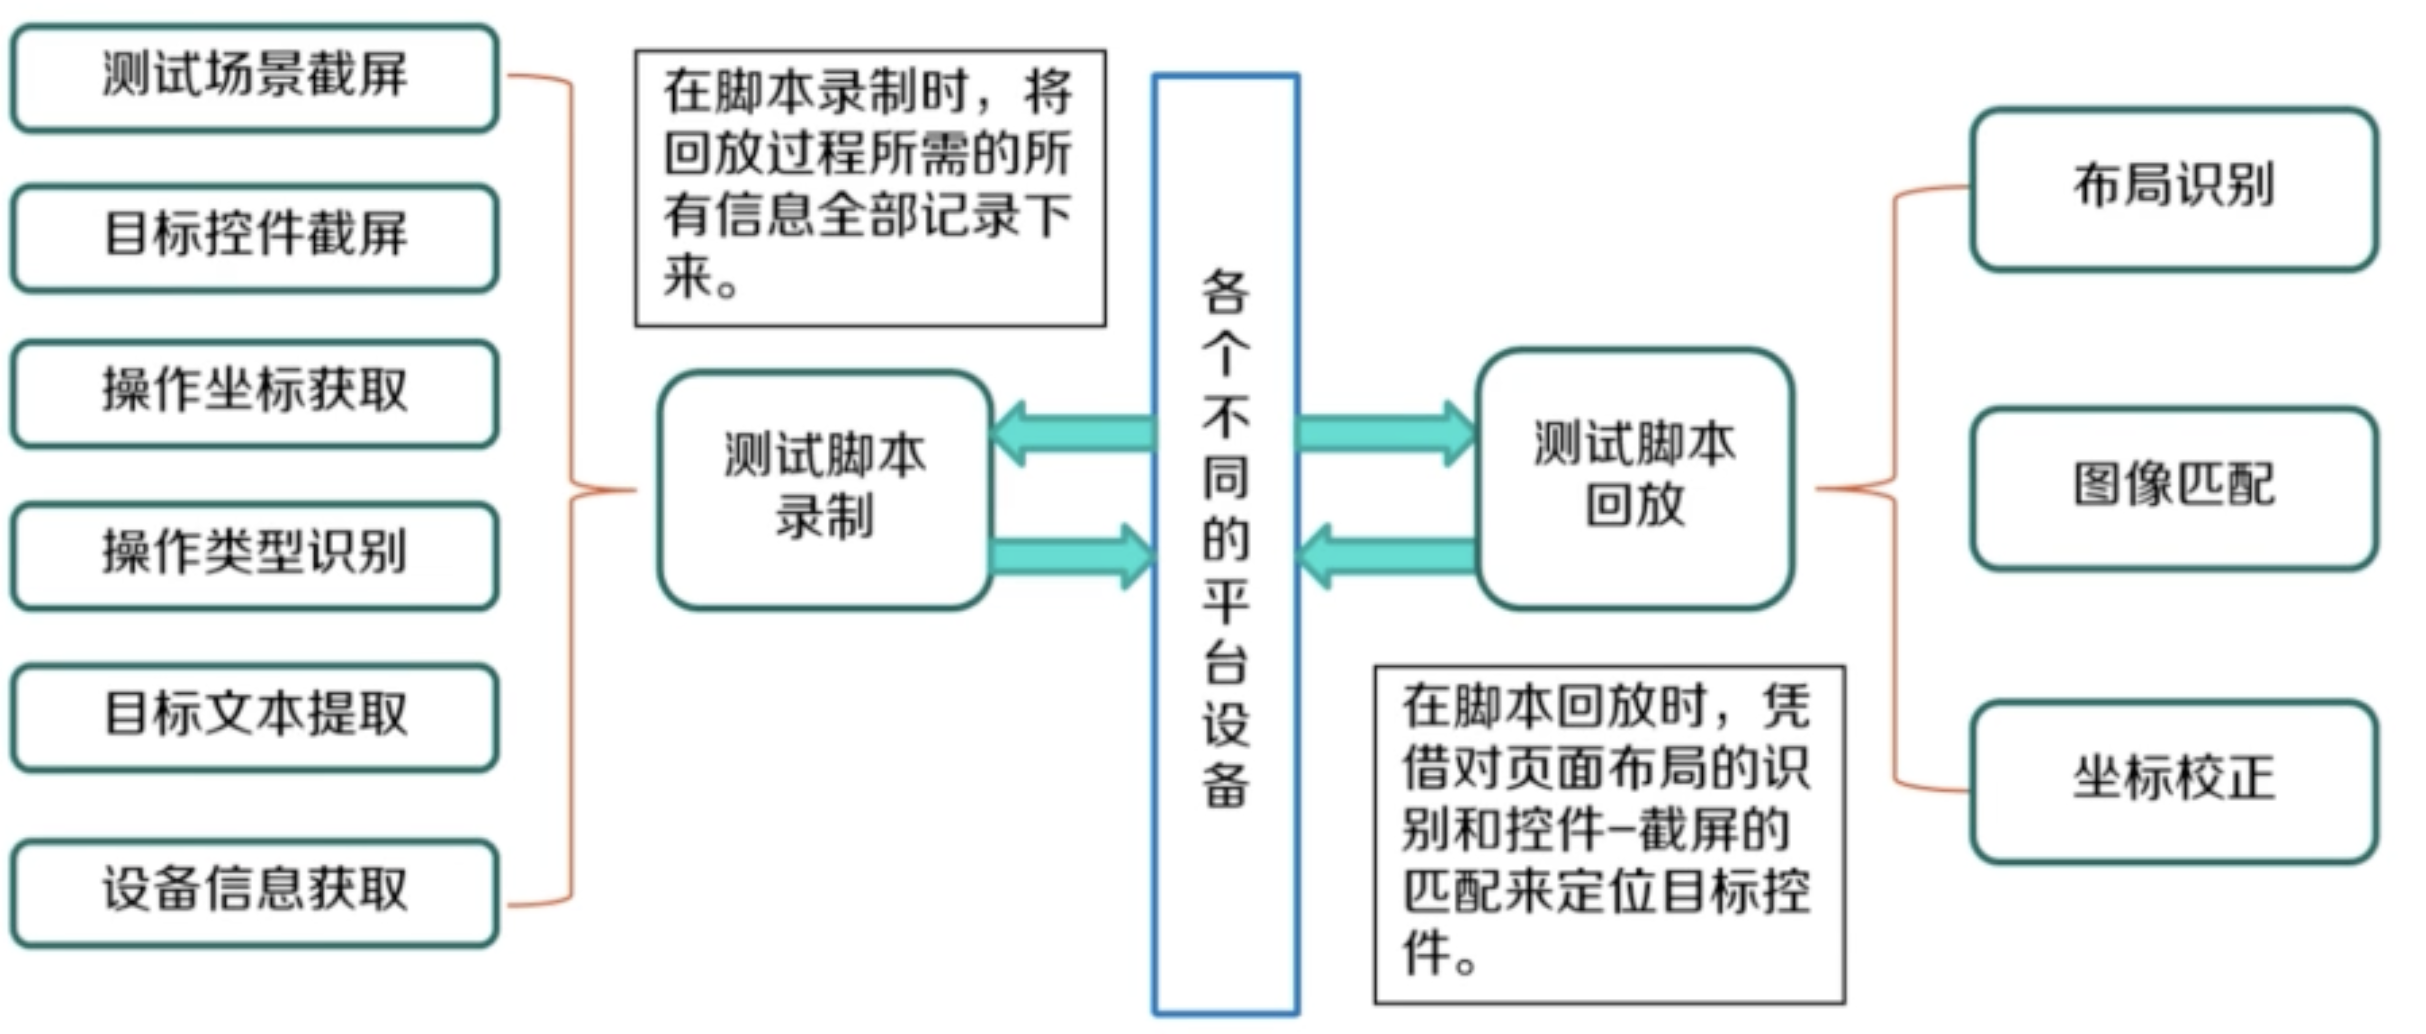
\includegraphics[width=0.8\textwidth]{images/脚本录制与回放的基本框架.png}
    \vspace{-1em}
\end{figure}

\subsection{跨平台的脚本结构}
\begin{figure}[H]
    \vspace{-0.5em}
	\centering
	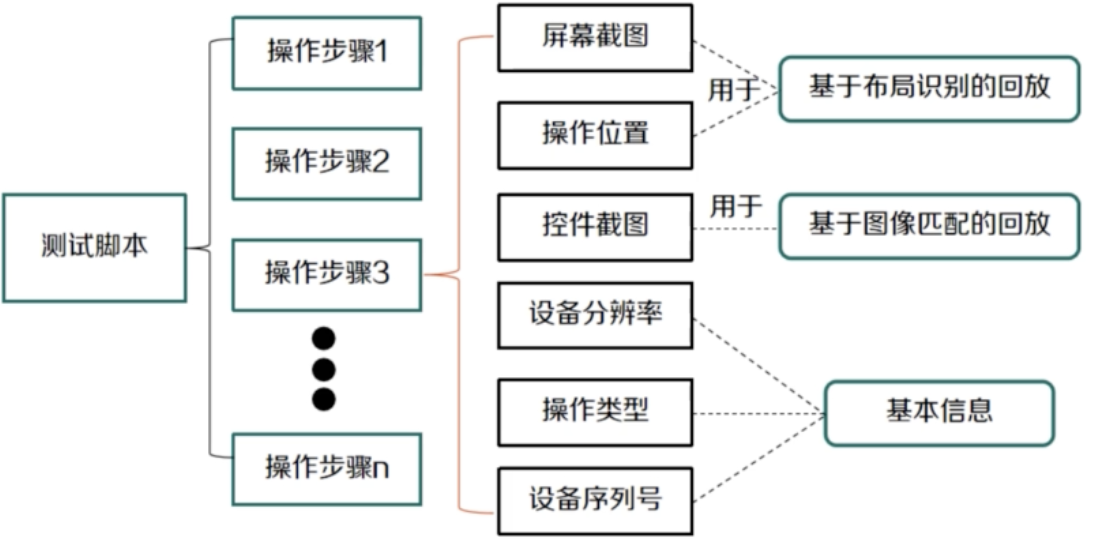
\includegraphics[width=0.7\textwidth]{images/跨平台的脚本结构.png}
    \vspace{-1em}
\end{figure}

\begin{itemize}
    \item 屏幕截图
    \begin{itemize}
        \item \verb|adb shell screencap -p <path>|\ 截屏截图
        \item \verb|adb pull sremote path> <local path>|\ 将手机中的文件\ \verb|<remote path>| \ 拷贝到PC的\ \verb|<local path>|
    \end{itemize}
    \item 控件截图
    \begin{itemize}
        \item \verb|adb shell uiautomator dump <path>|\ 获取界面布局
        \item \verb|adb pull|\ 命令将其拷贝到PC
        \item 利用操作的坐标定位控件,井将其从截图中截取出来
    \end{itemize}
    \item 操作类型、操作位置
    \begin{itemize}
        \item 通过前端JavaScript脚本的各类事件监听器
    \end{itemize}
    \item 设备分辨率、设备序列号
    \begin{itemize}
        \item \verb|AndroidDebugDridge.IDeviceChangeListener|
    \end{itemize}
\end{itemize}

\subsection{脚本的回放}

\subsubsection{图像特征比对}
\begin{figure}[H]
    \vspace{-0.5em}
	\centering
	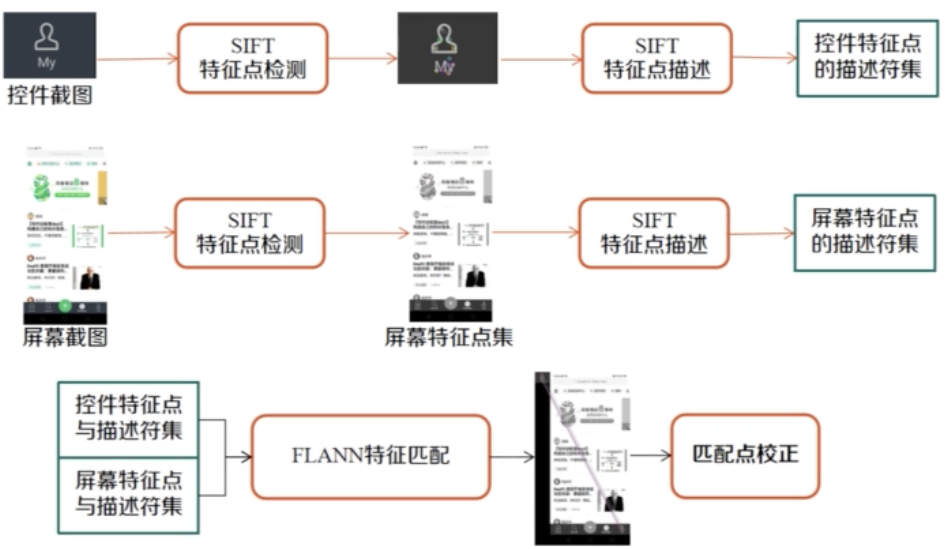
\includegraphics[width=0.8\textwidth]{images/图像特征比对.png}
    \vspace{-1em}
\end{figure}

\subsubsection{布局刻画}
\begin{itemize}
    \item 利用计算机视觉算法从GUI截图中找到所有控件的位置
    \item 利用OCR技术提取GUI截图中的文本
    \item 为所提取出来的控件划分控件组、行和列
\end{itemize}

\begin{figure}[H]
    \vspace{-0.5em}
	\centering
	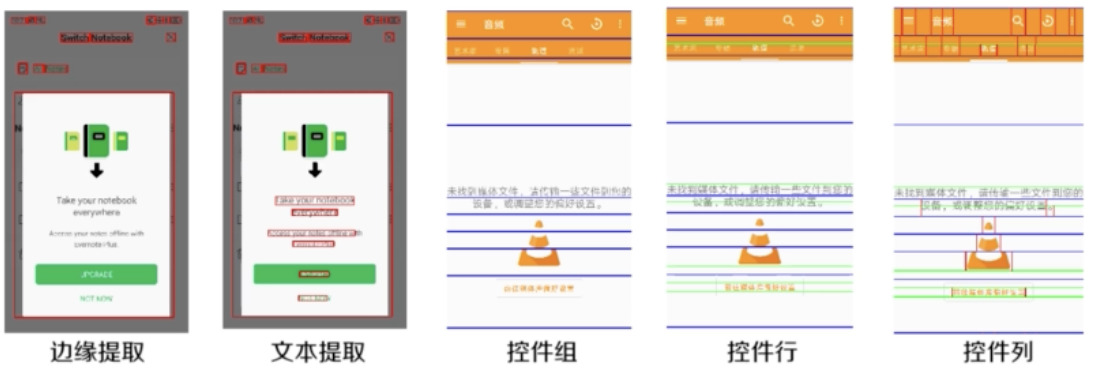
\includegraphics[width=0.85\textwidth]{images/布局刻画.png}
    \vspace{-1em}
\end{figure}

\subsubsection{坐标校正}
\begin{itemize}
    \item 基于布局识别的控件定位
    \begin{itemize}
        \item 容易受不同平台的外部布局的影响
        \item 不易受到图像变化的影响
    \end{itemize}
    \item 基于图像匹配的控件定位
    \begin{itemize}
        \item 容易受到图像变化的影响
        \item 不易受到不同平台的外部布局的影响
    \end{itemize}
    \item 为了结合二者的优点,提升算法的鲁棒性,引入了权重参数$\gamma$
    \begin{itemize}
        \item $W_{final} = \gamma \times W_{layout} + (1-\gamma) \times W_{image}$
        \begin{itemize}
            \item $W_{final}$:最终的控件定位
            \item $W_{layout}$:基于布局识别得到的控件定位
            \item $W_{image}$:基于图像匹配得到的控件定位
        \end{itemize}
    \end{itemize}
\end{itemize}

	\section{基于群智协同的众包测试}

\subsection{众包测试流程}
\begin{itemize}
    \item 申请上传:用广将自己的应用程序上传到众测平台,并指定相应的测试任务和酬劳信息。
    \item 任务选择和环境设置:众测人员自由选择他们想要完成的任务。选择后测试人员从平台上下载应用程序进行测试。
    \item 提交报告:众测人员根据选择的待测应用,对测试到的缺陷提交缺陷报告。
    \item 生成最终测试报告:平台收集补充信息,生成最终的缺陷报告,包括:一般信息、设备信息、操作路径等。
    \item 报告验证:客户将验证所有最终的缺陷报告,并决定如何酬劳每个提交报告的众包测试人员。
\end{itemize}

\begin{figure}[H]
    \vspace{-0.5em}
	\centering
	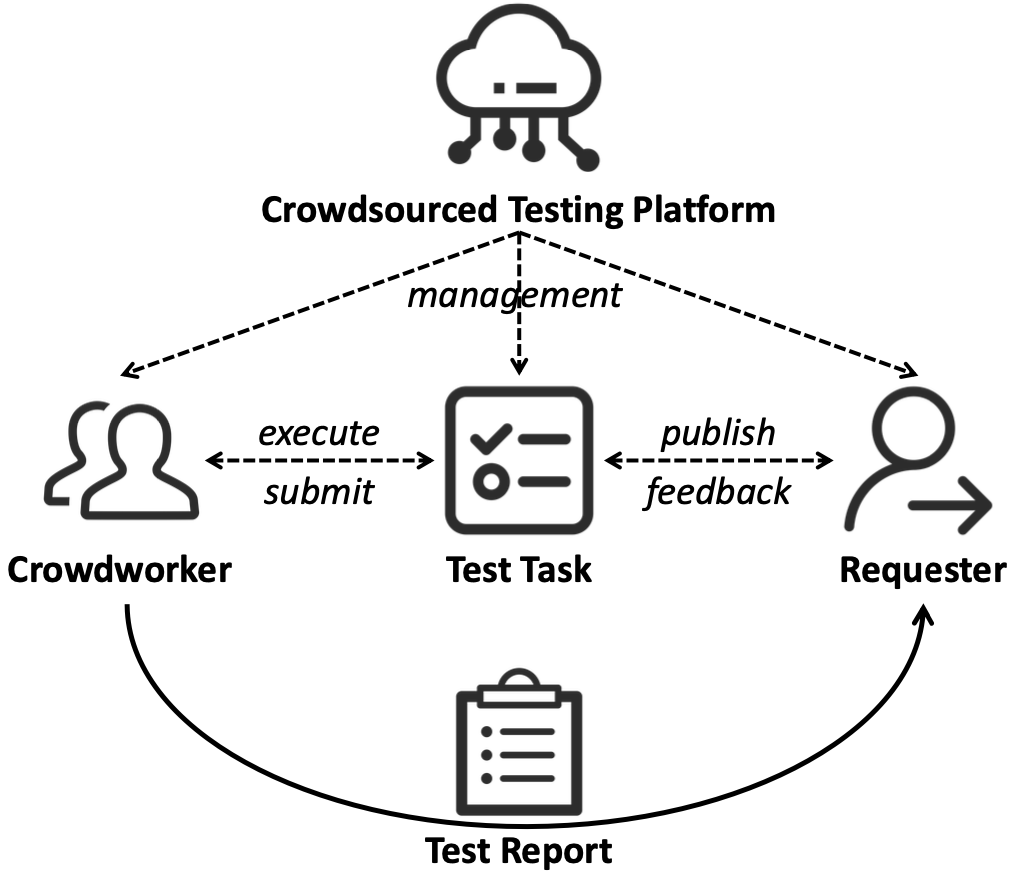
\includegraphics[width=0.4\textwidth]{images/众包测试流程.png}
    \vspace{-1em}
\end{figure}

\subsection{众包测试的特点}

众包测试的优势
\vspace{-0.5em}
\begin{multicols}{2}
    \begin{itemize}
        \item 更充分的测试时间
        \item 更广泛的测试方法
        \item 更多样的测试环境
        \item 更全面的测试覆盖
    \end{itemize}
\end{multicols}
\vspace{-1em}

众包测试面临的挑战
\vspace{-0.5em}
\begin{multicols}{2}
    \begin{itemize}
        \item 任务分配
        \item 任务奖励
        \item 众测过程引导
        \item 测试报告质量控制
    \end{itemize}
\end{multicols}
\vspace{-1em}

\subsection{对于众包测试存在的问题的解决}
协作式众包测试
\begin{itemize}
    \item 完成测试任务过程中进行信息共享与任务分配,用户在本系统中既承担测试任务也承担审核任务,充分利用用户协作,完成目标任务。
    \item 信息共享:用户在提交报告时进行实时相似报告推荐,避免重复报告提交。
    \item 任务分配:审核页面推荐待审核的报告列表,测试页面推荐待测页面。
    \item 协作方式:点赞点踩操作:利用用户的交叉审核,验证报告有效性。
    \item 一键Fork:Fork他人结果后进行修改,利用多人协作提升报告质量。
\end{itemize}

众测报告质量优化方法:文本和图像处理方法
\begin{itemize}
    \item 众测报告聚合
    \begin{itemize}
        \item Aggregator:对所有的测试报告做聚类,将相同的或相似的测试报告聚为同类。
        \item Summarizer:对每一类测试报告做整合,将其中的相关信息以可视化的方式最大化的呈现给开发者。
    \end{itemize}
    \item 众测报告排序
    \item 深度众测报告排序
    \item 众测报告半监督聚类
    \item 众测报告一致性检测
\end{itemize}



	\section{AI测试概述}

\subsection{智能软件和传统软件的区别}
\begin{itemize}
    \item 任务目标难以精确表达
    \item 非确定性开放环境运行
    \item 应用于复杂软硬件场景
    \item 输出的结果具有一定的随机性,AI测试的输出的结果与训练集的输入数据是非常相关的;而传统软件测试往往是有一个先验条件的,确定的输入能得到一个确定的输出
    \item 传统软件是由程序代码控制决策逻辑,而智能软件决策逻辑决由深度学习模型结构、训练后得到权重节点共同组成
\end{itemize}


\subsection{AI测试的难点}
\begin{itemize}
    \item 数据获取:对模型的训练和验证都需要大量的数据,如何获取到数据是一个最基本的问题。
    \item 数据质量:一般来说,数据质量越高,训练出的模型预测效果越好,如何评价和保障数据质量,是模型测试的另一个难点。
    \item 特征质量:特征直接影响到了模型的预测效果。特征维数过多,模型可能会过拟合;特征过少,模型可能会欠拟合。
    \item 结果验证:由于模型训练是黑盒形式,无法确认输入对应输出的逻辑是否准确。
    \item 线上服务效果验证:模型的测试不仅仅存在于上线前,随着时间的变化,模型的预测效果可能会出现偏差。如何实时跟踪这些变化,保证服务正常,也是需要关注的重点。
    \item 也存在不充分测试以及数据分布不均匀等问题
\end{itemize}

\subsection{图像扩增}
\begin{itemize}
    \item 基于图像处理的数据扩增
    \begin{itemize}
        \item 基于几何变换的扩增方法
        \begin{itemize}
            \item 旋转、缩放、平移、翻转、裁剪
        \end{itemize}
        \item 颜色空间变换:可以消除光照、亮度及色彩差异
        \begin{itemize}
            \item 亮度调整、对比度饱和度调整、颜色空间变换、色彩调整
        \end{itemize}
        \item 添加噪声和滤波
        \begin{itemize}
            \item 注入高斯噪声、椒盐噪声等;滤波:模糊、锐化等
        \end{itemize}
        \item 图像混合
        \item 随机擦除
    \end{itemize}
    \item 基于深度学习的数据扩增
    \begin{itemize}
        \item 基于GAN的数据增强:使用GAN生成模型来生成更多的数据,可用作解决类别不平衡问题的过采样技术
        \item 神经风格转换:通过神经网络风格迁移来生成不同风格的数据,防止模型过拟合
        \item AutoAugment
    \end{itemize}
\end{itemize}

\subsection{文本扩增}
\begin{itemize}
    \item 加噪(同义词替换、随机插入、随机替换、随机删除)以及回译
    \begin{itemize}
        \item 加噪:在原数据的基础 上通过替换词、删除词等方式创造和原数据相类
        似的新数据。
        \item 回译:将原有数据翻译为其他语言再翻译回原语言,由于语言逻辑顺序等的不同,回译的方法也往往能够得到和原数据差别较大的新数据。
    \end{itemize}
    \item 受限变分自编码器(CVAE),他是通过在回译的中间过程增加一些噪声,但增加过程很可能导致标签的变化,因此使用CVAE来同时考虑标签和文本来丰富中间过程的语言,最后可以翻译成原来的语言
    \item 文本生成、对抗生成
    \item 条件生成:使用模型判断可以替换的位置,然后再生成可以替换的词语
\end{itemize}

\subsection{公平性}
机器学习训练在涉及到性别、种族等与人相关的敏感属性时,常常会由于统计性偏差、算法本身甚至是人为偏见而引入歧视性行为。由此,为消除差别影响,改进机器学习公平性,主要途径包括提高训练数据集质量、改进算法降低对敏感属性的依赖以及定义指标量化和衡量歧视程度。\footnote{\url{https://blog.csdn.net/aizhushou/article/details/108724150}}

\subsection{后门攻击}
深度学习中的后门攻击通过后门模型学习攻击者选择的子任务和(良性)主任务的方式向DL模型植入后门:\footnote{\url{https://zhuanlan.zhihu.com/p/541578519}}
\begin{itemize}
    \item 一方面,对于不包含触发器的输入input,后门模型表现得与干净模型一样正常,因此仅通过检查测试样本的测试准确性来区分后门模型和干净模型是不可能的;
    \item 另一方面,一旦秘密触发器Trigger(只有攻击者知道)出现在输入中,后门模型就会被错误引导去执行攻击者的子任务,比如分类任务中将输入分类到攻击者指定的目标类别。
\end{itemize}

	\section{模糊测试}

\subsection{模糊测试的背景与提出}
模糊测试的提出背景:测试的局限性
\begin{itemize}
    \item 输入空间庞大,无法穷举所有测试用例
    \item 实现逻辑复杂,无法覆盖所有场景
    \item 测试语言未知,无法判定测试的预期输出
\end{itemize}

模糊测试是一种通过向目标程序提供非预期的输入并监视异常结果来发现软件漏洞的方法
\begin{itemize}
    \item 大数定律的典型应用:通过随机生成测试数据,只要测试次数足够多,概率低的偶然事件就会发生
\end{itemize}

\subsection{模糊测试框架}

\begin{figure}[H]
    \vspace{-0.5em}
    \subfloat{
        \begin{minipage}[t]{0.25\linewidth}
        \centering
        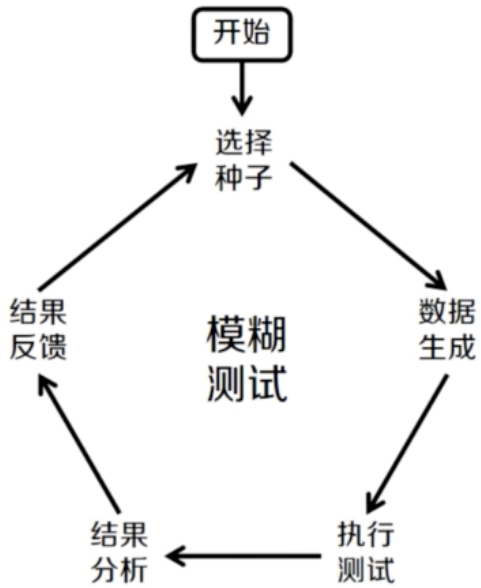
\includegraphics[width=0.97\linewidth]{images/模糊测试流程.png}
        \end{minipage}
    }
    \hspace{1em}
    \subfloat{
	    \begin{minipage}[t]{0.7\linewidth}
	    \centering
	    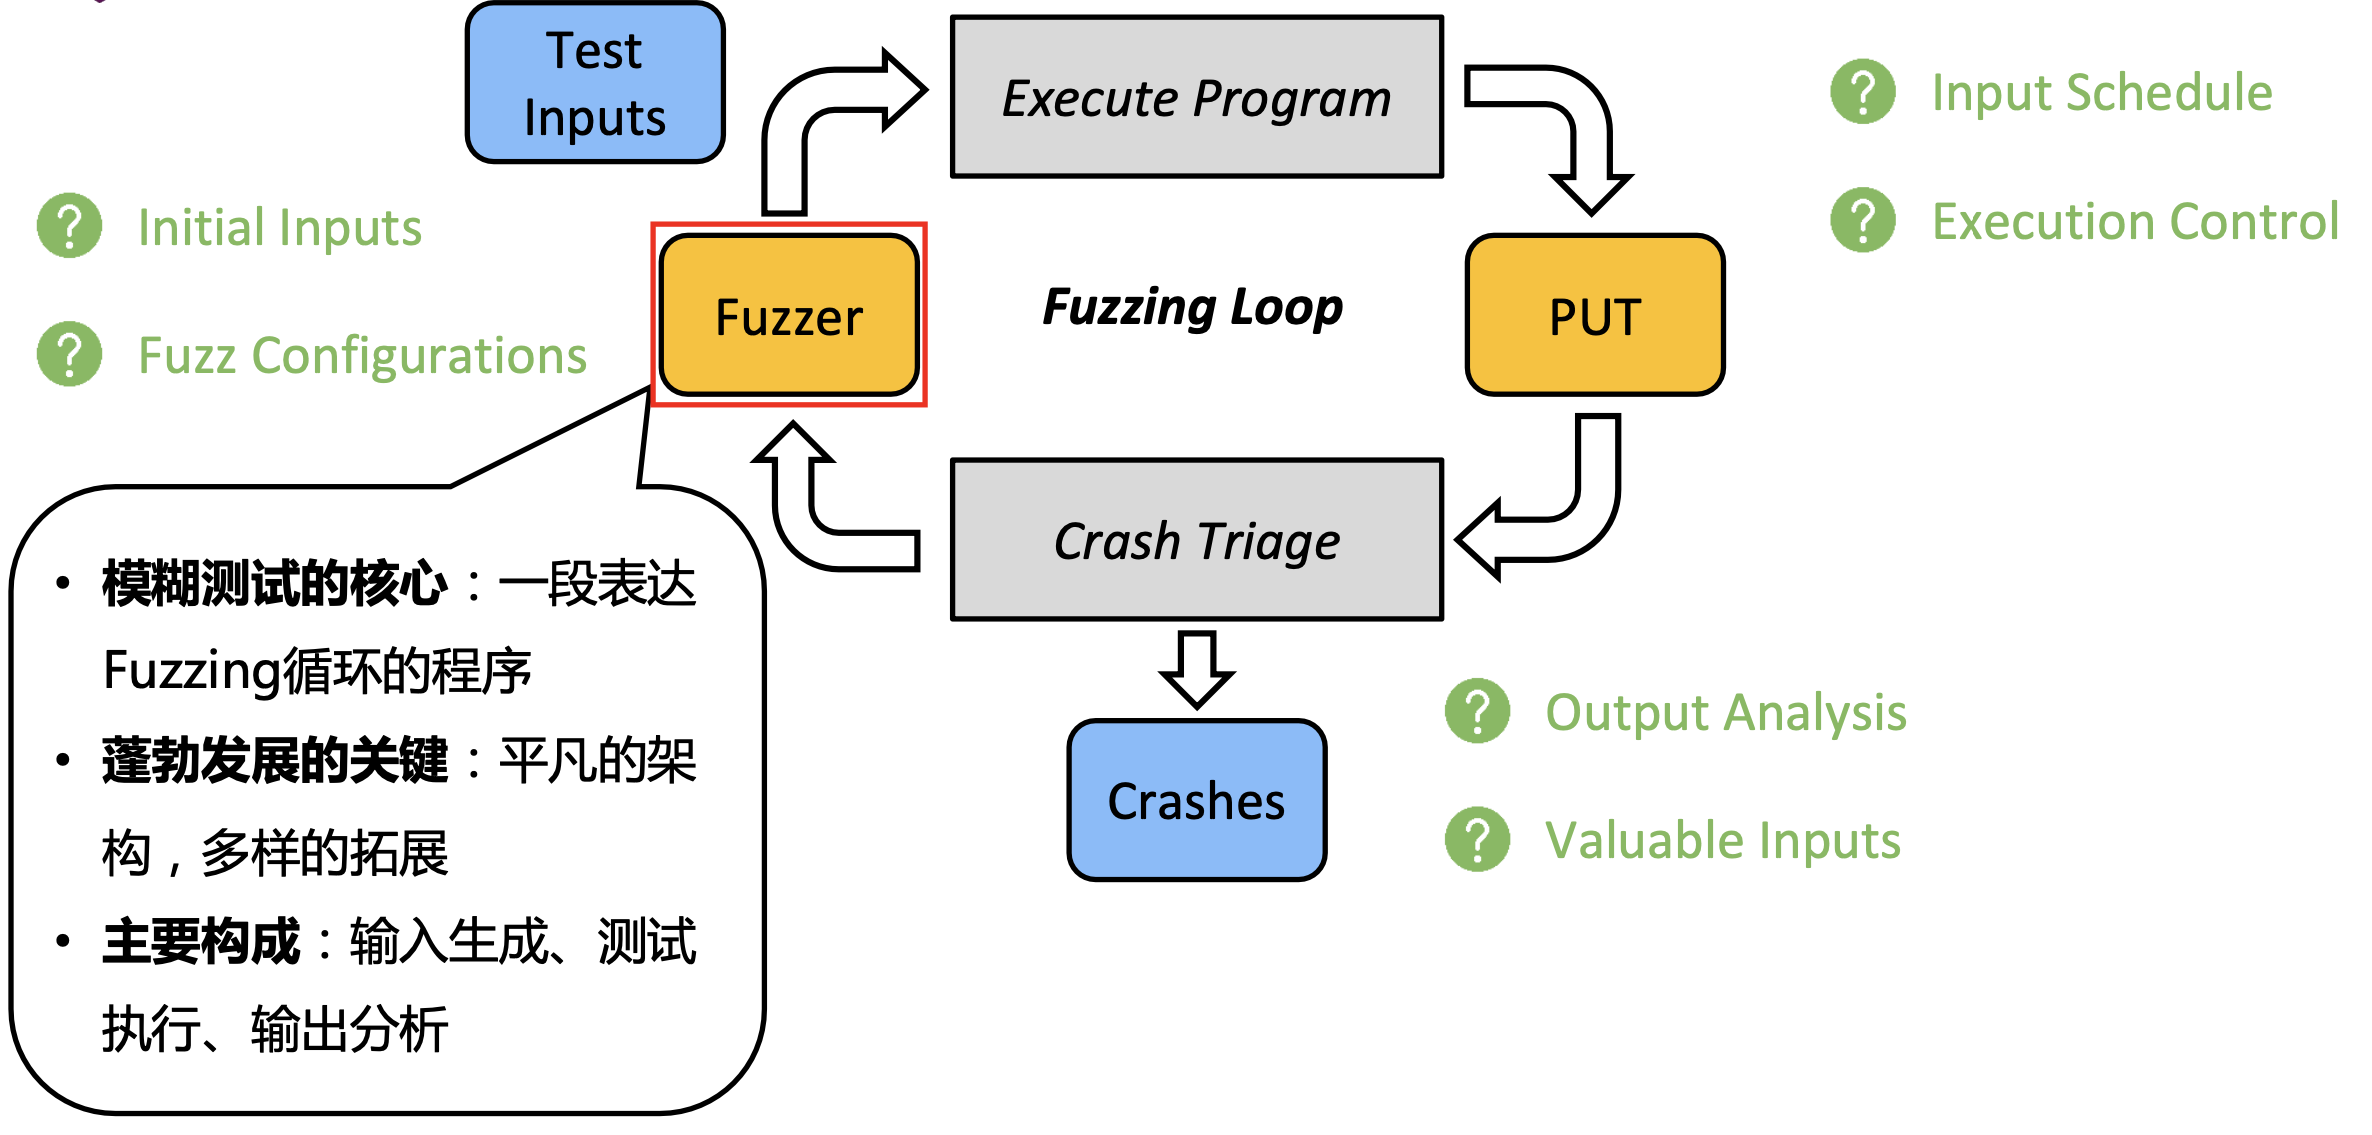
\includegraphics[width=0.97\linewidth]{images/模糊测试框架1.png}
	    \end{minipage}
	}
\end{figure}

\begin{figure}[H]
    \vspace{-0.5em}
	\centering
	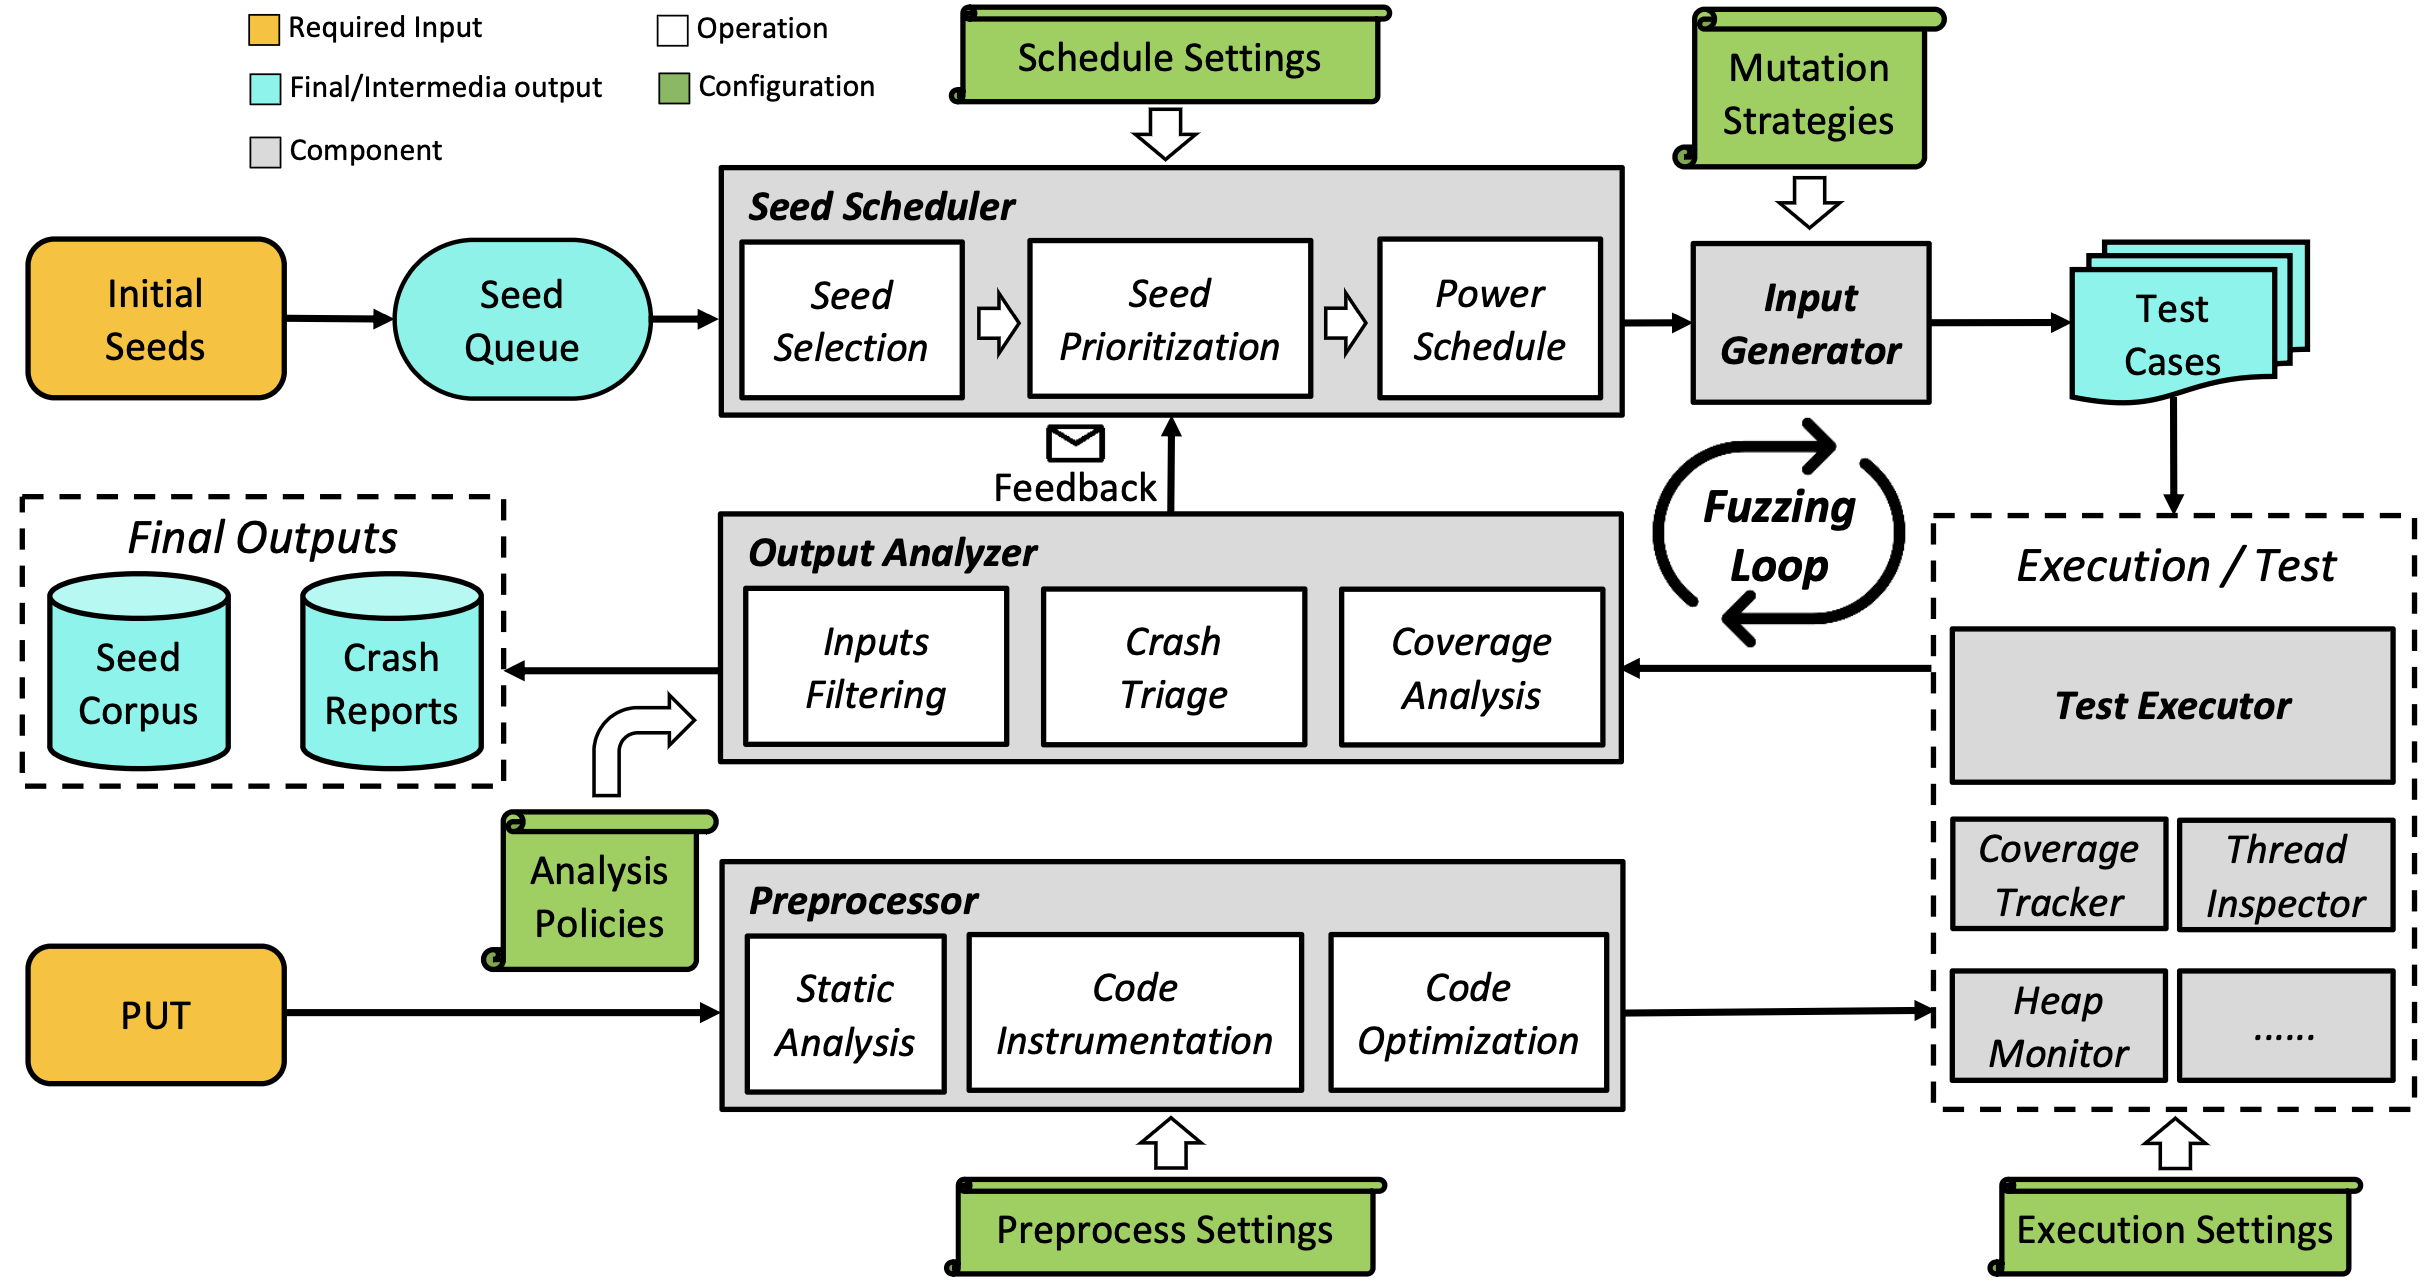
\includegraphics[width=0.85\textwidth]{images/模糊测试框架2.png}
    \vspace{-1em}
\end{figure}

模糊测试监测内容:程序中的哪些现象能够帮助判断是否存在问题
\vspace{-0.5em}
\begin{multicols}{2}
    \begin{itemize}
        \item 断言失败
        \item 异常崩溃
        \item 无效输入
        \item 错误输出
    \end{itemize}
\end{multicols}
\vspace{-1em}

\subsection{基于灰盒的模糊测试流程}
\begin{figure}[H]
    \vspace{-0.5em}
	\centering
	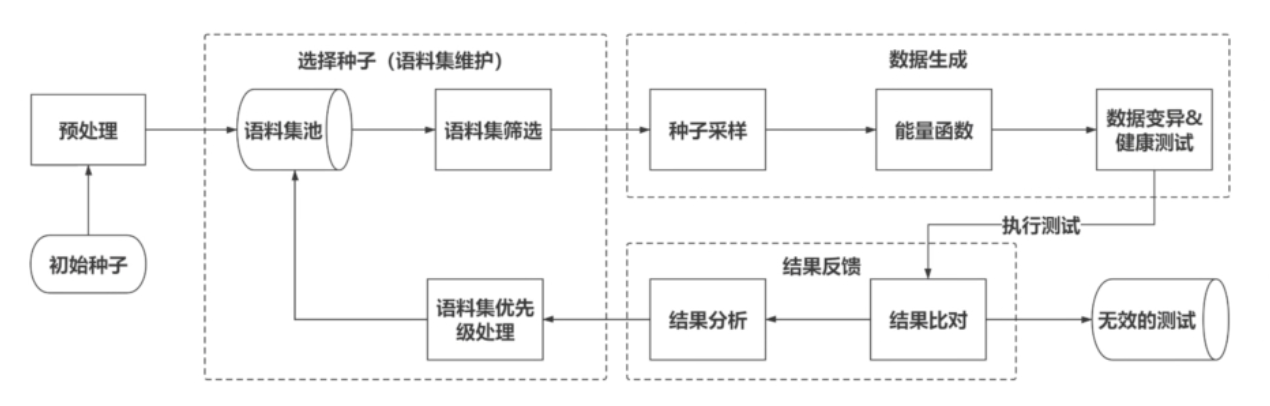
\includegraphics[width=0.95\textwidth]{images/基于灰盒的模糊测试流程.png}
    \vspace{-1em}
\end{figure}

\begin{itemize}
    \item 初始种子:已有的测试用例或者已知的符合所要测试程序输入范围的数据 
    \item 预处理:种子经过一定的预处理(比如编码转换或图像裁剪)使得种子满足程序的输入条件或参数要求
    \item 语料集:由于对测试用例数量和质量的要求,一般会将种子打包形成语料集
    \item 种子采样:根据模糊测试变异方法从送入过程引导的语料集中形成符合变异方法输入的种子元组
    \item 能量函数:旨在通过对语料集进行变异成功率检测实现在同样的测试计算资源尽可能生成多的能够成功变异的测试数据 
    \item 数据变异:根据所选用的变异方法,对选取的原始测试数据施加扰动,生成新的测试输入
    \item 与结果参照物(理论上应该得到的结果)对比或者是否发生崩溃
    \begin{itemize}
        \item 大多数情况用覆盖率分析来指导语料集的进一步优化
    \end{itemize}
\end{itemize}

AI模糊测试流程与传统模糊测试流程类似
\begin{itemize}
    \item 结果反馈和结果分析都由深度学习模型提供
    \item 模型同时指导语料集的维护
\end{itemize}

\subsection{算子差分模糊测试}
方法:将差分测试与模糊测试相结合
\begin{itemize}
    \item 引入值运算运用于算子接口,首先针对每个新生成测试用例,分别获取算子接口的中间过程值和返回值。
    \item 接着对输入参数、中间值和返回值进行处理。
    \item 然后对Tensor数据采用加权求和进行降维,井结合基本类型参数,最终得到一组覆盖值。
    \item 最后将新用例的一组覆盖值与语料集中所有已有元素的覆盖值进行比较,如果最近距离大于某个阈值,则将新用例加入语料集。
    \item 在差分测试的指导下,通过不同框架间的距离标准或精度标准来测量算子接口的结果。
\end{itemize}


\end{document}


